\documentclass[10pt,spanish,aspectratio=1610]{beamer}
\usepackage[utf8]{inputenc}
\usepackage{amsmath}
\usepackage{graphicx}
\usepackage{amssymb}
\usepackage{multicol}
\usepackage[spanish]{babel}
\spanishdecimal{.}
\usepackage{subfig}
\usepackage{fancyhdr}
\usepackage{pstricks}
\usepackage{color}
\usepackage[ruled]{algorithm2e}
\usepackage{listings}
\usepackage{xcolor}
\usepackage{gensymb}

\definecolor{graywhite}{rgb}{0.9529,0.9607,0.9686}
\definecolor{bluegray}{rgb}{0.6823, 0.7411, 0.8}
\definecolor{darkred}{rgb}{0.7372, 0.2392, 0.2392}
\definecolor{bluedark}{rgb}{0.294, 0.4705, 0.6407}
\definecolor{darkgreen}{rgb}{0.1764, 0.5294, 0.0901}
\lstset{
  backgroundcolor=\color{graywhite},   % choose the background color; you must add \usepackage{color} or \usepackage{xcolor}; should come as last argument
  basicstyle=\footnotesize,        % the size of the fonts that are used for the code
  breakatwhitespace=false,         % sets if automatic breaks should only happen at whitespace
  breaklines=true,                 % sets automatic line breaking
  captionpos=b,                    % sets the caption-position to bottom
  commentstyle=\color{darkgreen},    % comment style
  keepspaces=true,                 % keeps spaces in text, useful for keeping indentation of code (possibly needs columns=flexible)
  keywordstyle=\color{darkred},       % keyword style
  language=Octave,                 % the language of the code
  morekeywords={*,...},            % if you want to add more keywords to the set
  numbers=left,                    % where to put the line-numbers; possible values are (none, left, right)
  numbersep=7pt,                   % how far the line-numbers are from the code
  numberstyle=\tiny\color{bluedark}, % the style that is used for the line-numbers
  showspaces=false,                % show spaces everywhere adding particular underscores; it overrides 'showstringspaces'
  showstringspaces=false,          % underline spaces within strings only
  showtabs=false,                  % show tabs within strings adding particular underscores
  stepnumber=1,                    % the step between two line-numbers. If it's 1, each line will be numbered
  stringstyle=\color{bluedark},     % string literal style
  frame=single,
  rulecolor=\color{bluegray},
  tabsize=2,                   % sets default tabsize to 2 spaces
  xleftmargin=1cm,
  xrightmargin=0.5cm,
  framexleftmargin=0.5cm,
  extendedchars=true,
  literate={á}{{\'a}}1 {é}{{\'e}}1 {í}{{\'i}}1 {ó}{{\'o}}1 {ú}{{\'u}}1 {Á}{{\'A}}1 {É}{{\'E}}1 {Í}{{\'I}}1 {Ó}{{\'O}}1 {Ú}{{\'U}}1,
}

\DeclareMathOperator{\atantwo}{atan2}
\setbeamercolor{block title}{fg=white,bg=blue!70!black}
\setbeamercolor{block body}{fg=black, bg=blue!10!white}
\setbeamertemplate{blocks}[rounded][shadow=false]
\setbeamercovered{transparent}
\beamertemplatenavigationsymbolsempty
\setbeamertemplate{frametitle}{
  \leavevmode
  \hbox{\begin{beamercolorbox}[wd=0.85\paperwidth,left]{frametitle}
    \usebeamerfont{frametitle}\insertframetitle
  \end{beamercolorbox}
%  \begin{beamercolorbox}[wd=0.25\paperwidth,center]{frametitle}
%    \usebeamerfont{frametitle}\hfill\hspace*{5ex}\footnotesize{\insertsubsection}
%  \end{beamercolorbox}
}}
\setbeamertemplate{footline}{
  \leavevmode%
  \hbox{%
    \begin{beamercolorbox}[colsep=-0.5pt,wd=.33\paperwidth,ht=3ex,dp=1.5ex,center]{author in head/foot}%
      \usebeamerfont{author in head/foot}\insertshortauthor~~ (\insertshortinstitute)
    \end{beamercolorbox}%
    \begin{beamercolorbox}[colsep=-0.5pt,wd=.34\paperwidth,ht=3ex,dp=1.5ex,center]{date in head/foot}%
      \usebeamerfont{author in head/foot}\insertshorttitle
    \end{beamercolorbox}%
    \begin{beamercolorbox}[colsep=-0.5pt,wd=.33\paperwidth,ht=3ex,dp=1.5ex,right]{author in head/foot}%
      \usebeamerfont{author in head/foot}\insertsection{}\hspace*{2em}\scriptsize{\insertframenumber{}}\hspace*{1ex}
    \end{beamercolorbox}
  }
}
\setbeamersize
{
    text margin left=0.25cm,
    text margin right=0.25cm
}

\begin{document}
\renewcommand{\tablename}{Tabla}
\renewcommand{\figurename}{Figura}

\title[@Home Basics 2024-1]{Tareas Básicas en Robots de Servicio Doméstico}
\author[Marco Negrete]{Marco Negrete}
\institute[FI, UNAM]{Facultad de Ingeniería, UNAM}
\date[2o Workshop ]{2o Workshop de Sistemas Ciberfísicos}

\begin{frame}
\titlepage
\end{frame}

\section{Introducción}
\begin{frame}\frametitle{Presentación del curso}
  \textbf{Objetivos:}
  \begin{itemize}
  \item Aprender los conceptos básicos para operar un robot móvil autónomo
  \item Implementar dichos conceptos en un ambiente simulado
  \item Familiarizar al estudiante con la plataforma ROS
  \end{itemize}
\end{frame}

\begin{frame}\frametitle{Contenido}
  \begin{enumerate}
  \item Introducción y generalidades
    \begin{itemize}
    \item Componentes básicos de un robot móvil
    \item Herramientas de software para el desarrollo de robots móviles
    \end{itemize}
  \item Planeación de movimientos
    \begin{itemize}
    \item El problema de la planeación de movimientos
    \item Mapas geométricos y topológicos
    \item Celdas de ocupación y diagramas de Voronoi
    \item Planeación de rutas mediante búsqueda en grafos
    \item Modelos cinemáticos: diferencial, omnidireccional, Ackermann
    \item Control de posición y seguimiento de trayectorias
    \item Campos potenciales artificiales
    \end{itemize}
  \item Mapeo y localización
    \begin{itemize}
    \item Localización mediante filtro de Kalman extendido
    \item Localización mediante filtros de partículas
    \item Creación de mapas mediante agrupamiento
    \item Localización y mapeo simultáneos
    \end{itemize}
  \end{enumerate}
\end{frame}

\begin{frame}\frametitle{Contenido}
  \begin{enumerate}
    \setcounter{enumi}{3}
  \item Conceptos básicos de visión artificial
    \begin{itemize}
    \item Imágenes y espacios de color
    \item Operadores morfológicos
    \item Extracción de características geométricas
    \item Reconocimiento mediante redes neuronales artificiales
    \item Nubes de puntos
    \end{itemize}
  \item Conceptos básicos de manipulación
    \begin{itemize}
    \item Movimiento de cuerpo rígido
    \item Cinemática directa
    \item Cinemática inversa por métodos numéricos
    \item Planeación y seguimiento de trayectorias
    \end{itemize}
  \item Herramientas para la interacción humano-robot
    \begin{itemize}
    \item Síntesis de voz con la biblioteca Festival
    \item Reconocimiento de voz con la biblioteca CMU Sphinx
    \item Reconocimiento de gestos con la biblioteca OpenPose
    \end{itemize}
  \end{enumerate}
\end{frame}

\begin{frame}\frametitle{Contenido}
  \textbf{Bibliografía recomendada:}
  \begin{itemize}
    \item \url{https://drive.google.com/drive/folders/1gb7VQJG5eUkCvCginRHHGn5lez6VASBJ?usp=sharing}
    \item \url{https://drive.google.com/drive/folders/1Epl2b51xEJzCvzfugBD1i7xGdKYdJucy?usp=sharing}
  \end{itemize}
  
\end{frame}


\section{Introducción y generalidades (2023-08-17)}
\begin{frame}\frametitle{Contexto y definiciones}
  \begin{itemize}
  \item La palabra \textit{robot} tiene su origen en la obra \textit{Rossum's Universal Robots} del escritor checo $Karel \,\check{C}apeck$, publicada en 1921, y su significado es ``trabajo duro''.
  \item Latombe (1991) define un robot como un dispositivo mecánico versátil equipado con sensores y actuadores bajo el control de un sistema de cómputo \cite{Latombe1991MotionPlanning}.
  \item Arkin (1998) propone que un robot inteligente es una máquina capaz de extraer información de su ambiente y usar el conocimiento acerca de su mundo para moverse de manera segura y significativa, con un propósito específico \cite{Arkin1998BehBasedRobo}.
  \item Robótica es la ciencia que estudia la conexión inteligente entre la percepción y la acción. 
  \end{itemize}
\end{frame}

\begin{frame}\frametitle{Áreas de la Robótica}
  
  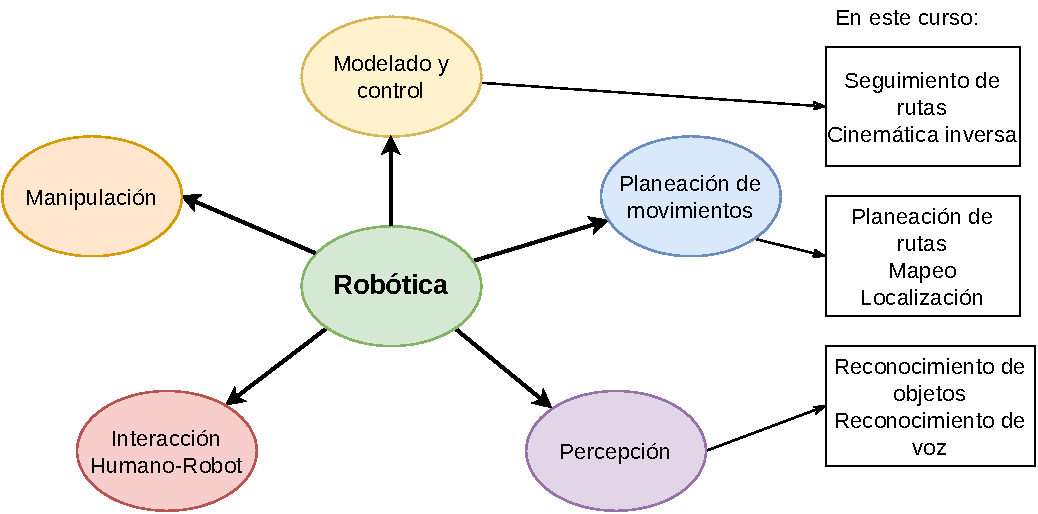
\includegraphics[width=0.9\textwidth]{Figures/RoboticsAreas.pdf}
\end{frame}

\begin{frame}\frametitle{Componentes de un robot}
  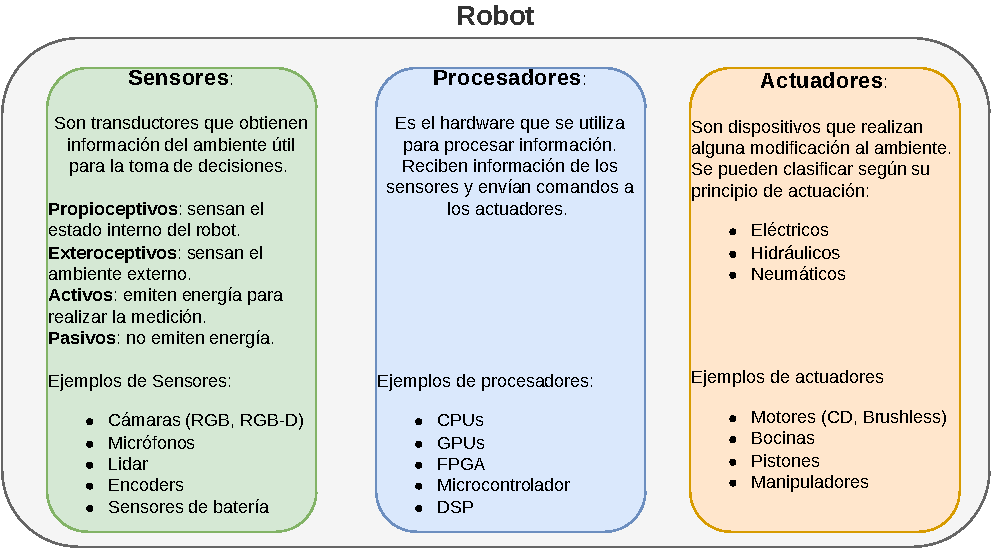
\includegraphics[width=0.9\textwidth]{Figures/RobotComponents.pdf}
\end{frame}

\begin{frame}\frametitle{Conceptos Básicos}
  \begin{itemize}
  \item \textbf{Configuración:} es la descripción de la posición en el espacio de todos los puntos del robot. Se denota con $q$.
  \item \textbf{Espacio de configuraciones:} es el conjunto $Q$ de todas las posibles configuraciones. 
  \item \textbf{Grados de libertad:} número mínimo de variables independientes para describir una configuración. En este curso, la base móvil del robot tiene 3 GdL, la cabeza tiene 2 GDL y cada brazo tiene 7 GDL más 1 GdL para el gripper. En total, el robot tiene 21 GdL. 
  \end{itemize}
  \textbf{Propiedades del robot:}
  \begin{itemize}
  \item \textbf{Holonómico:} el robot puede moverse instantáneamente en cualquier dirección del espacion de configuraciones. Comunmente se logra mediante ruedas de tipo \textit{Mecanum} u \textit{Omnidireccionales}. 
  \item \textbf{No holonómico:} existen restricciones de movimiento en velocidad pero no en posición. Son restricciones que solo se pueden expresar en términos de la velocidad pero no pueden integrarse para obtener una restricción en términos de posición. Ejemplo: un coche sólo puede moverse en la dirección que apuntan las llantas delanteras, sin embargo, a través de maniobras puede alcanzar cualquier posición y orientación. El robot de este curso es no holonómico. 
  \end{itemize}
\end{frame}

\begin{frame}\frametitle{Conceptos Básicos}
  \textbf{Propiedades de los algoritmos:}
  \begin{itemize}
  \item \textbf{Complejidad:} cuánta memoria y cuánto tiempo se requiere para ejecutar un algoritmo, en función del número de datos de entrada (número de grados libertad, número de lecturas de un sensor, entre otros).
  \item \textbf{Optimalidad:} un algoritmo es óptimo cuándo encuentra una solución que minimiza una función de costo.
  \item \textbf{Completitud:} un algoritmo es completo cuando garantiza encontrar la solución siempre que ésta exista. Si la solución no exite, indica falla en tiempo finito.
    \begin{itemize}
    \item Completitud de resolución: la solución existe cuando se tiene una discretización. 
    \item Completitud probabilística: la probabilidad de encontrar la solución tiende a 1.0 cuando el tiempo tiende a infinito.
    \end{itemize}
  \end{itemize}
  Una explicación más detallada se puede encontrar en el Cap. 3 de \cite{choset2005principles}.
\end{frame}


%%%%%%%%%%%%%%%%%%%
%%% 2023-08-22 %%%%
%%%%%%%%%%%%%%%%%%%
\section{La plataforma ROS (2023-08-22)}
\begin{frame}\frametitle{La plataforma ROS}
  
\includegraphics[width=0.3\textwidth]{Figures/Ros_logo.png}
  \[\]
  \textbf{ROS (Robot Operating System) } es un \textit{middleware} de código abierto para el desarrollo de robots móviles.
  \begin{itemize}
  \item Implementa funcionalidades comúnmente usadas en el desarrollo de robots como el paso de mensajes entre procesos y la administración de paquetes.
  \item Muchos drivers y algoritmos ya están implementados.
  \item Es una plataforma distribuida de procesos (llamados \textit{nodos}).
  \item Facilita el reuso de código.
  \item Independiente del lenguaje (Python y C++ son los más usados).
  \item Facilita el escalamiento para proyectos de gran escala. 
  \end{itemize}
\end{frame}

\begin{frame}\frametitle{Conceptos}
  ROS se puede entender en dos grandes niveles conceptuales:
  \begin{itemize}
  \item \textbf{Sistema de archivos:} Recursos de ROS en disco
  \item \textbf{Grafo de procesos:} Una red \textit{peer-to-peer} de procesos (llamados nodos) en tiempo de ejecución.
  \end{itemize}
\end{frame}

\begin{frame}\frametitle{Sistema de archivos}
  \begin{columns}
    \begin{column}{0.5\textwidth}
      Recursos en disco:
      \begin{itemize}
      \item \textbf{Workspace:} carpeta que contiene los paquete desarrollados
      \item \textbf{Paquetes:} Principal unidad de organización del software en ROS (concepto heredado de Linux)
      \item \textbf{Manifiesto:} (\texttt{package.xml}) provee metadatos sobre el paquete (dependencias, banderas de compilación, información del desarrollador)
      \item \textbf{Mensajes (msg):} Archivos que definen la estructura de un \textit{mensaje} en ROS.
        \item \textbf{Servicios (srv):} Archivos que definen las estructuras de la petición (\textit{request}) y respuesta (\textit{response}) de un servicio. 
      \end{itemize}
    \end{column}
    \begin{column}{0.4\textwidth}
      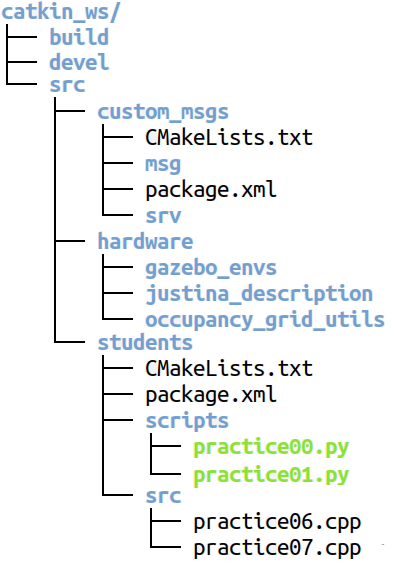
\includegraphics[width=\textwidth]{Figures/catkin_tree.png}
    \end{column}
  \end{columns}
\end{frame}

\begin{frame}\frametitle{Grafo de procesos}
  El grafo de procesos es una red \textit{peer-to-peer} de programas (nodos) que intercambian información entre sí. Los principales componentes del este grafo son:
  \[\]
  \begin{columns}
    \begin{column}{0.5\textwidth}
      \begin{itemize}
      \item master
      \item servidor de parámetros
      \item nodos
      \item mensajes
      \item servicios 
      \end{itemize}
    \end{column}
    \begin{column}{0.5\textwidth}
      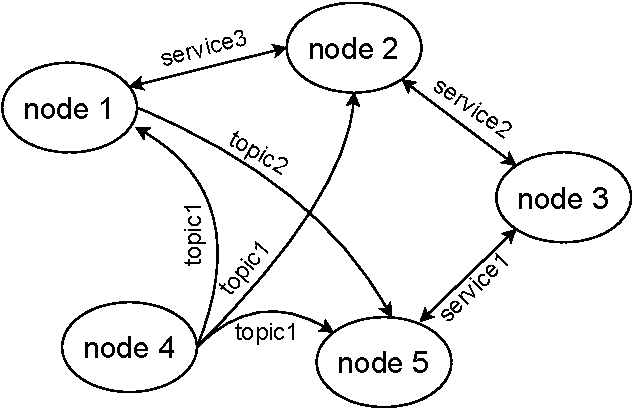
\includegraphics[width=\textwidth]{Figures/RosGraph.pdf}
    \end{column}
  \end{columns}
\end{frame}

\begin{frame}\frametitle{Tópicos y servicios}
  Los nodos (procesos) en ROS intercambian información a través de dos grandes patrones:
  \begin{columns}
    \begin{column}{0.6\textwidth}
        \begin{itemize}
        \item \textbf{Tópicos}
          \begin{itemize}
          \item Son un patrón $1:n$ de tipo \textit{publicador/suscriptor}
          \item Son no bloqueantes
          \item Utilizan estructuras de datos definidas en archivos \texttt{*.msg} para el envío de información
          \end{itemize}
        \item \textbf{Servicios}
          \begin{itemize}
          \item Son un patrón $1:1$ de tipo \textit{petición/respuesta}
          \item Son bloqueantes
          \item Utilizan estructuras de datos definidas en archivos \texttt{*.srv} para el intercambio de información. 
          \end{itemize}
        \end{itemize}
    \end{column}
    \begin{column}{0.4\textwidth}
      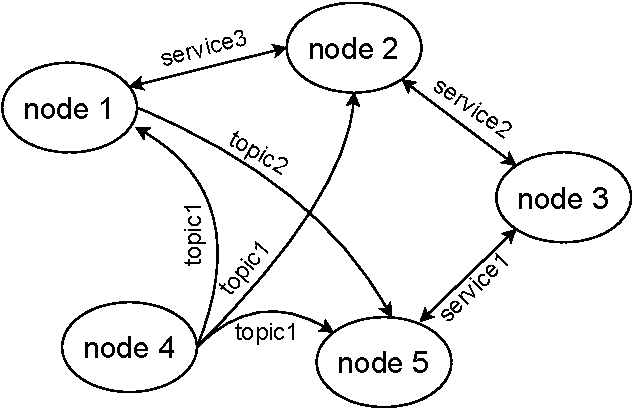
\includegraphics[width=\textwidth]{Figures/RosGraph.pdf}
    \end{column}
  \end{columns}
  \[\]
  Para mayor información:
  \begin{itemize}
  \item Tutoriales \url{http://wiki.ros.org/ROS/Tutorials}
  \item Koubâa, A. (Ed.). (2020). Robot Operating System (ROS): The Complete Reference. Springer Nature
  \end{itemize}
\end{frame}

\begin{frame}\frametitle{El simulador Gazebo}
  
\end{frame}

\begin{frame}[containsverbatim]\frametitle{Tarea 02 - La plataforma ROS}
  \begin{enumerate}
  \item Investigar aplicaciones de ROS y el simulador Gazebo. Se pueden consultar las siguientes páginas:
    \begin{itemize}
    \item https://www.openrobotics.org/markets
    \item https://vimeo.com/649649866/37198994b5
    \item https://robots.ros.org/robonaut2/
    \item https://github.com/nasa/astrobee
    \end{itemize}
  \item Buscar para qué sirven los comandos: \texttt{rosrun}, \texttt{rostopic list} y \texttt{rostopic echo}
  \item Abra el archivo \texttt{catkin\_ws/src/students/scripts/assignment02.py} y agregue el siguiente código en la línea 25:
    \begin{lstlisting}[language=Python,firstnumber=25]
n = int((msg.angle_max - msg.angle_min)/msg.angle_increment/2)
obstacle_detected = msg.ranges[n] < 1.0
  \end{lstlisting}
  En el mismo archivo, en la línea 45, agregue el siguiente código:
  \begin{lstlisting}[language=Python,firstnumber=45]
msg_cmd_vel = Twist()
msg_cmd_vel.linear.x = 0 if obstacle_detected else 0.3
pub_cmd_vel.publish(msg_cmd_vel)
  \end{lstlisting}
  \end{enumerate}
\end{frame}

\begin{frame}[containsverbatim]\frametitle{Tarea 02 - La plataforma ROS}
  \begin{enumerate}
    \setcounter{enumi}{3}
  \item Abra una terminal y corra la simulación con el comando (revise las instrucciones en el README del repositorio):
    \begin{verbatim}
   roslaunch surge_et_ambula justina_gazebo.launch
\end{verbatim}
  \item En otra terminal, corra la tarea 2 con el comando:
    \begin{verbatim}
   rosrun students assignment02.py
\end{verbatim}
  \item Observe el comportamiento y describa lo que sucede. De preferencia, elabore un diagrama de flujo que describa el comportamiento del robot.
  \end{enumerate}
  \[\]
  \textbf{Entregables:}
  \begin{itemize}
  \item Código modificado en la rama correspondiente del repositorio en línea.
  \item Documento escrito con todos los puntos anteriores. 
  \end{itemize}
  \textbf{Deadline: } 2023-08-31 al inicio de la clase. 
\end{frame}



%%%%%%%%%%%%%%%%%%%
%%% 2023-08-24 %%%%
%%%%%%%%%%%%%%%%%%%
\section{Planeación de movimientos (2023-08-24)}

\begin{frame}\frametitle{Planeación de movimientos}
  El problema de la planeación de movimientos comprende cuatro tareas principales:
  \begin{itemize}
  \item Navegación: encontrar un conjunto de puntos $q \in Q_{free}$ que permitan al robot moverse desde una configuración inicial $q_{start}$ a una configuración final $q_{goal}$. 
  \item Mapeo: construir una representación del ambiente a partir de las lecuras de los sensores y la trayectoria del robot. 
  \item Localización: determinar la configuración $q$ dado un mapa y lecturas de los sensores. 
  \item Barrido: pasar un actuador por todos los puntos $q\in Q_b \subset Q$.
  \end{itemize}
\end{frame}

\section{Representación del ambiente (2023-08-24)}
\begin{frame}\frametitle{Representación del ambiente}
  Un mapa es cualquier representación del ambiente útil en la toma de decisiones.
  \begin{itemize}
  \item Interiores (se suelen representar en 2D)
    \begin{itemize}
    \item Celdas de ocupación
    \item Mapas de líneas
    \item Mapas topológicos: Diagramas de Voronoi generalizados. 
    \item Mapas basados en \textit{Landmarks}
    \end{itemize}
  \item Exteriores (suelen requerir una representación 3D)
    \begin{itemize}
    \item Celdas de elevación
    \item Celdas de ocupación 3D
    \item Octomaps
    \end{itemize}
  \end{itemize}
\end{frame}

\begin{frame}\frametitle{Celdas de ocupación}
  Es un tipo de mapa geométrico. El espacio se discretiza con una resolución determinada y a cada celda se le asigna un número $p\in[0,1]$ que indica su nivel de ocupación. En un enfoque probabilístico este número se puede interpretar como la certeza que se tiene de que una celda esté ocupada.
  \begin{figure}
    \centering
    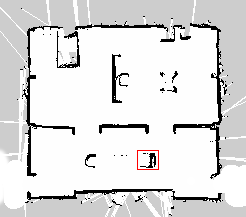
\includegraphics[width=0.4\textwidth]{Figures/OccupancyGrid.png}
    
\includegraphics[width=0.4\textwidth]{Figures/UniversumZoom.png}
    \end{figure}
  El mapa resultante se representa en memoria mediante una matriz de valores de ocupación. En ROS, los mapas utilizan el mensaje \texttt{nav\_msgs/OccupancyGrid}.
\end{frame}

\begin{frame}\frametitle{Inflado de celdas de ocupación}
  Aunque las celdas de ocupación representan el espacio donde hay obstáculos y donde no, en realidad, el robot no puede posicionarse en todas las celdas libres, debido a su tamaño, como se observa en la figura:
  \begin{columns}
    \begin{column}{0.6\textwidth}
      \begin{figure}
        \centering
        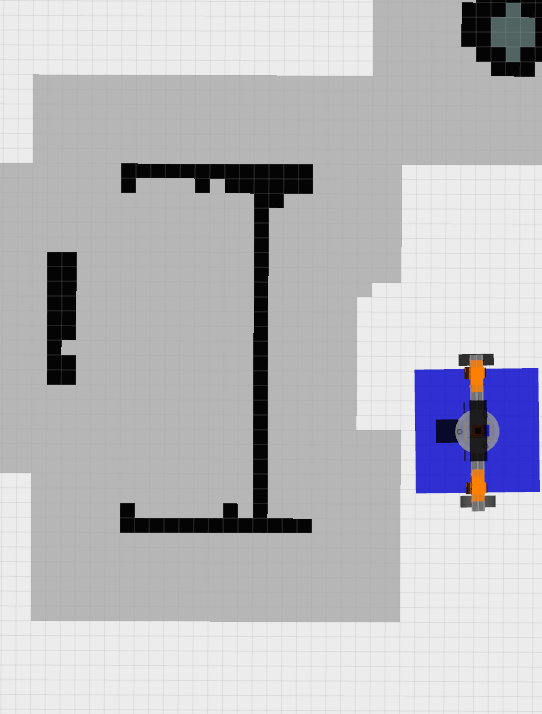
\includegraphics[width=0.45\textwidth]{Figures/InflationExample1.png}
        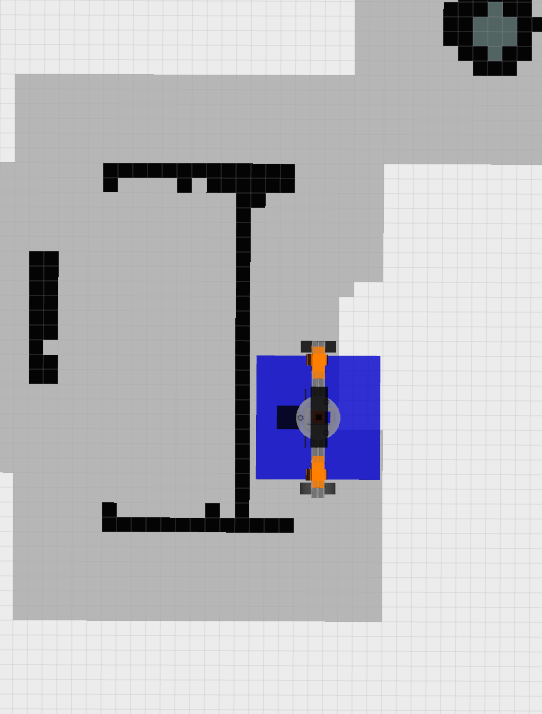
\includegraphics[width=0.45\textwidth]{Figures/InflationExample2.png}
      \end{figure}
    \end{column}
    \begin{column}{0.4\textwidth}
      \begin{itemize}
      \item Celdas blancas: espacio libre.
      \item Celdas negras: espacio con obstáculos.
        \item Celdas grises: espacio sin obstáculos donde el robot no puede estar debido a su tamaño. 
      \end{itemize}
    \end{column}
  \end{columns}
  \begin{itemize}
  \item Un mapa de celdas de ocupación debe \textit{inflarse} antes de usarse para planear rutas.
  \item Esta operación se conoce como \textit{dilatación} y es un operador morfológico como se verá en la sección de conceptos de visión.
  \item El inflado se usa para planeación de rutas, no para localización.
  \end{itemize}
\end{frame}

\begin{frame}\frametitle{Inflado de celdas de ocupación}
  \label{fr:inflation}
  \begin{algorithm}[H]
    \DontPrintSemicolon
    \KwData {\;
      Mapa $M$ de celdas de ocupación\;
      Radio de inflado $r_i$
    }
    \KwResult{Mapa inflado $M_{inf}$}
    $M_{inf} = $ Copia de $M$\;
    \ForEach{$i\in [0,\dots,rows)$}
      {
        \ForEach{$j\in [0,\dots,cols)$}
          {
            //Si la celda está ocupada, marcar como ocupadas las $r_i$ celdas de alrededor.\;
            \If{$M[i,j] == 100$ }
               {
                 \ForEach{$k_1\in [-r_i,\dots,r_i]$}
                   {
                     \ForEach{$k_2\in [-r_i,\dots,r_i]$}
                       {
                         $M_{inf}[i+k_1, j+k_2] = 100$
                       }
                   }
               }    
          }
        }
        \label{alg:inflation}
        \caption{Algoritmo de inflado de mapas}
  \end{algorithm}
\end{frame}

\begin{frame}\frametitle{Mapas de líneas}
  También son mapas geométricos, pero al almancenar \textit{features} requieren mucho menos memoria. La desventaja es la dificultad para extraer líneas del ambiente y la poca precisión en el empatado. 
  \begin{figure}
    \centering
    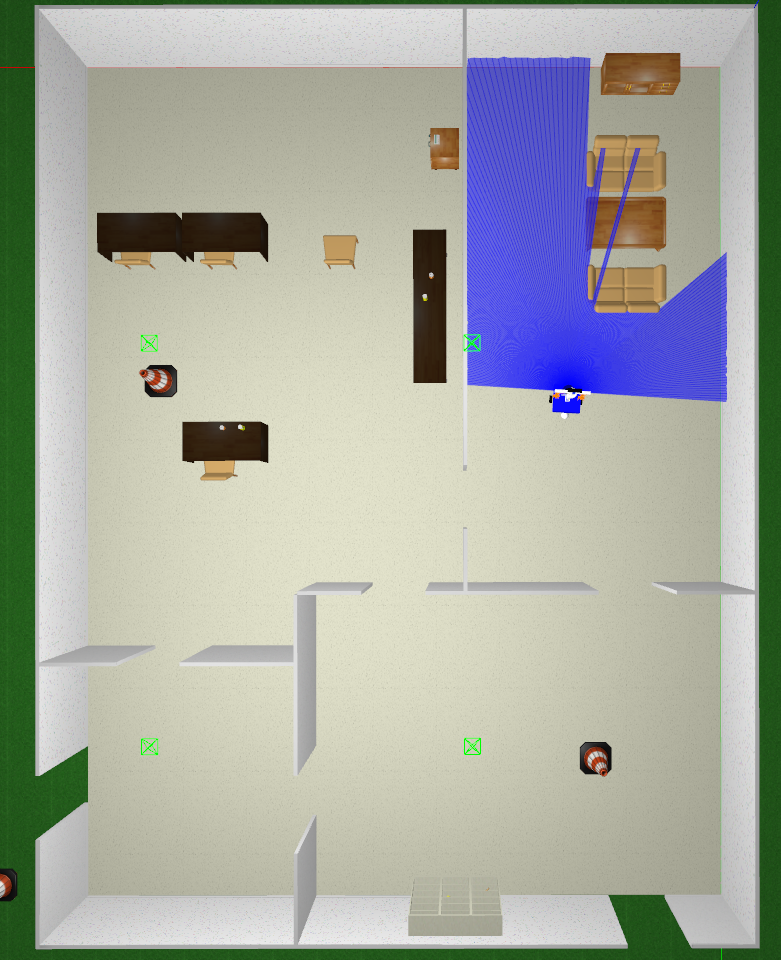
\includegraphics[width=0.3\textwidth]{Figures/MapLinesGazebo.png}
    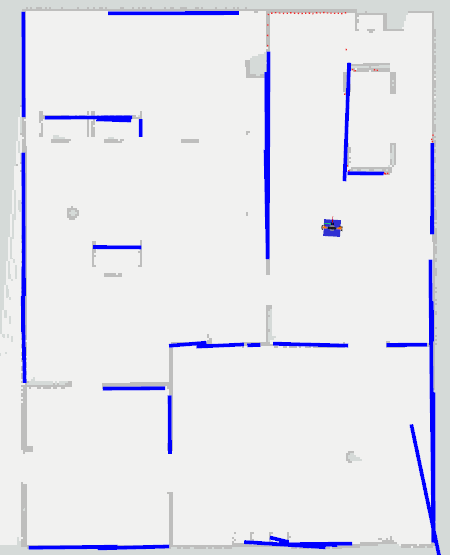
\includegraphics[width=0.3\textwidth]{Figures/MapLines.png}
  \end{figure}
  Algunos métodos para extraer líneas:
  \begin{itemize}
  \item \textit{Split and merge}
  \item Transformada Hough (se verá en la sección de visión computacional)
  \item RANSAC
  \end{itemize}
\end{frame}

\begin{frame}\frametitle{Algoritmo \textit{Split and Merge}}
  Se utiliza principalmente cuando los datos provienen de un sensor Lidar y por lo tanto, los puntos están en secuencia.
  \[\]
  \begin{columns}
    \begin{column}{0.65\textwidth}
      \begin{algorithm}[H]
        \DontPrintSemicolon
        \KwData {Conjunto de puntos $P$}
        \KwResult{Conjunto de líneas en forma normal $(\rho, \theta$)}
        \;
        Ajustar una recta $L$ al conjunto $P$ por mínimos cuadrados\;
        Encontrar el punto $p_i$ más lejano a la recta\;
          \uIf{$d(p_i, L) > d_{0}$}
             {
               Dividir $P$ en dos subconjuntos $P_1$ y $P_2$ usando $p_i$ como pivote\;
               Aplicar este algoritmo recursivamente para $P_1$ y $P_2$\;
               Devolver las rectas de ambos subconjuntos
             }
             \Else
                 {
                   Devolver la recta $L$ en forma normal $(\rho, \theta)$\;
                 }
                 \caption{\textit{Split}}
        \end{algorithm}
    \end{column}
    \begin{column}{0.35\textwidth}
      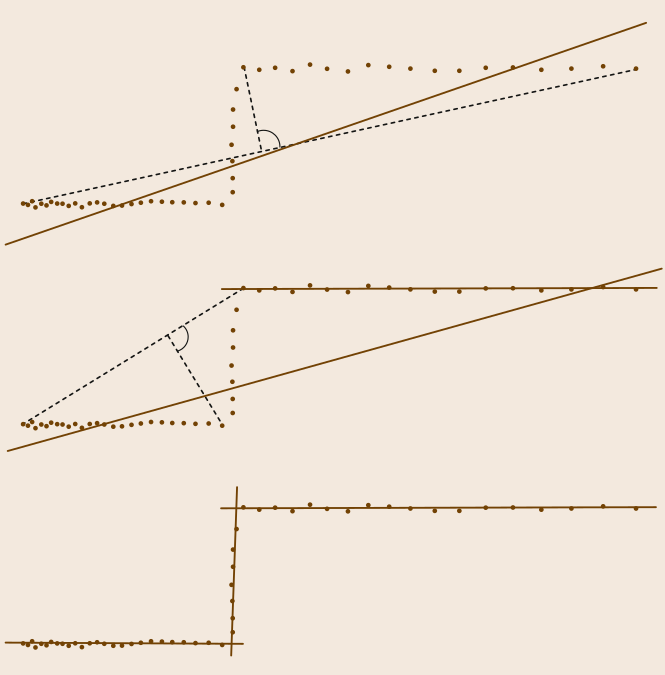
\includegraphics[width=\textwidth]{Figures/SplitAndMerge.png}
    \end{column}
  \end{columns}
\end{frame}

\begin{frame}\frametitle{Algoritmo \textit{Split and Merge}}
  \label{fr:split_merge}
  El algoritmo anterior realiza la partición (\textit{split}) del conjunto de puntos en posibles rectas y obtiene la ecuación para cada conjunto por mínimos cuadrados. La etapa de mezcla (\textit{merge}) consiste simplemente en considerar como una sola recta, dos segmentos con parámetros $(\rho, \theta)$ similares. Los parámetros a sintonizar en este algoritmo son:
  \begin{itemize}
  \item $d_0$ : umbral de distancia entre un punto $p_i$ y la recta $L$
  \item $N_{min}$ : número mínimo de puntos para considerar que un subconjunto puede ser una recta.
  \item $\rho_{tol}$ : valor máximo de diferencia entre dos rectas con $\rho_1$ y $\rho_2$ para considerarlas como una sola recta.
  \item $\theta_{tol}$ : valor máximo de diferencia entre dos rectas con $\theta_1$ y $\theta_2$ para considerarlas como una sola recta. 
  \end{itemize}
\end{frame}

\begin{frame}\frametitle{Mínimos cuadrados}
  Este método busca minimizar las distancias entre los puntos $(x_i,y_i)$ y la recta en forma normal dada por los parámetros $(\rho, \theta)$.
  \[\]
  Dado un conjunto de puntos $(x_i, y_i)$, la recta $(\rho,\theta)$ que mejor se ajusta se puede obtener con:
  \begin{eqnarray*}
    \theta &=& \frac{1}{2}\atantwo\left(-2\sum_i (\bar{x} - x_i)(\bar{y}-y_i)\quad,\quad \sum_i\left[(\bar{y} - y_i)^2 - (\bar{x} - x_i)^2\right]\right)\\
    \rho &=& \bar{x}\cos\theta + \bar{y}\sin\theta
  \end{eqnarray*}
  con
  \begin{eqnarray*}
    \bar{x} &=& \frac{1}{n}\sum_i x_i\\
    \bar{y} &=& \frac{1}{n}\sum_i y_i
  \end{eqnarray*}
\end{frame}

\begin{frame}\frametitle{Diagrama de Voronoi Generalizado}
  \begin{itemize}
  \item A diferencia de los mapas geométricos, donde se busca reflejar la forma exacta del ambiente, los \textbf{mapas topológicos} buscan representar solo las relaciones espaciales de los puntos de interés.
  \item Los Diagramas de Voronoi dividen el espacio en regiones. Cada región está asociada a un punto llamado semilla, sitio o generador. Una región asociada a una semilla $x$ contiene todos los puntos $p$ tales que $d(x,p)$ es menor o igual que la distancia $d(x^\prime, p)$ a cualquier otra semilla $x^\prime$.
  \item Un diagrama de Voronoi generalizdo (GVD) considera que las semillas pueden ser objetos con dimensiones y no solo puntos. 
  \end{itemize}
  \begin{figure}
    \centering
    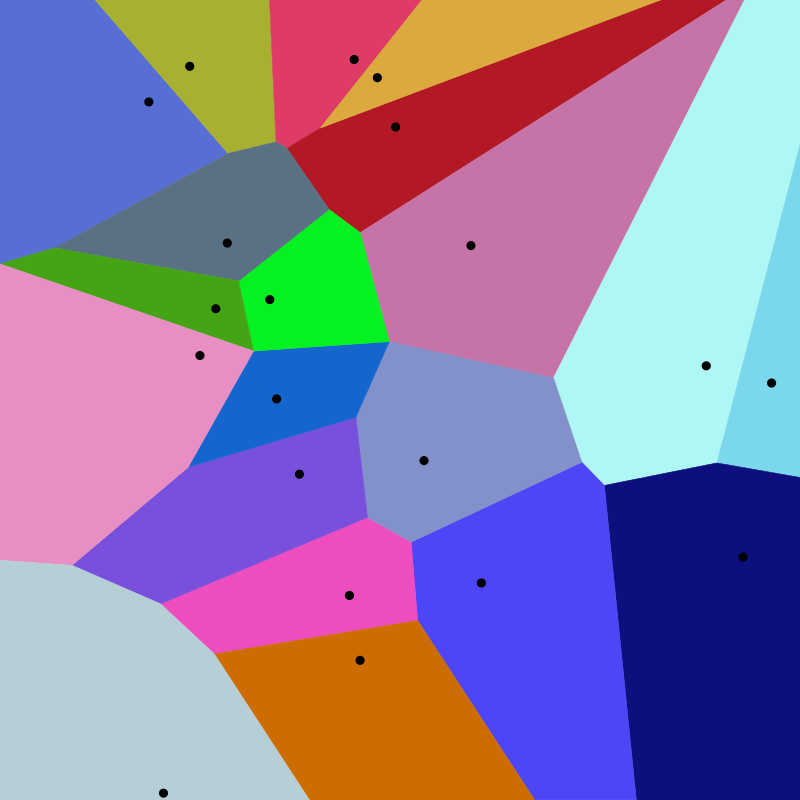
\includegraphics[height=0.4\textheight]{Figures/GVD.png}
    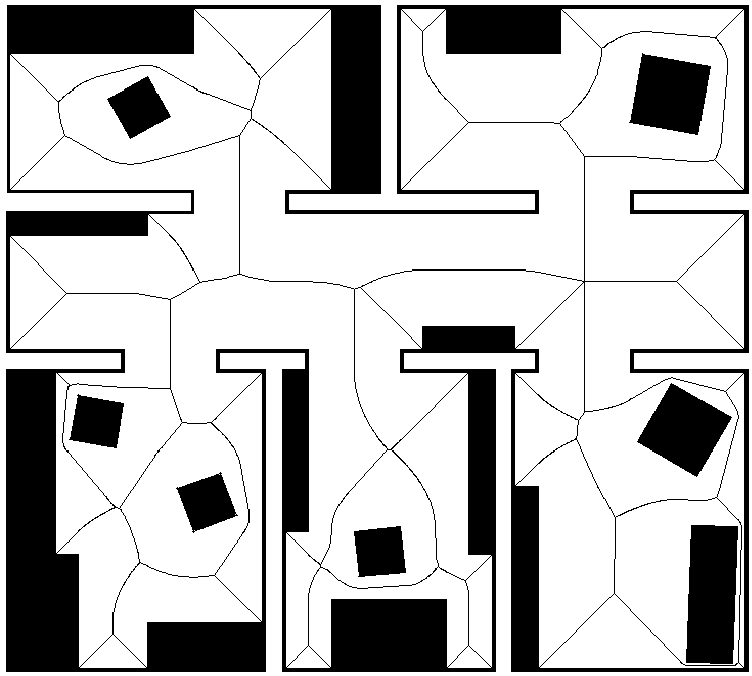
\includegraphics[height=0.4\textheight]{Figures/GVDExample.png}
  \end{figure}
  \begin{itemize}
    \item La forma de las regiones depende de la función de distancia que se utilice. 
  \end{itemize}
\end{frame}

\begin{frame}\frametitle{El algoritmo \textit{Brushfire}}
  \begin{columns}
    \begin{column}{0.65\textwidth}
      \begin{itemize}
      \item Obtener un GVD es aún un problema abierto
      \item Se simplifica el problema si se asume que el espacio está representado por Celdas de Ocupación
      \item En este caso el GVD se puede obtener mediante el algoritmo \textit{Brushfire}
      \item El mapa de rutas mostrado en la figura se forma con las celdas que son máximos locales en el mapa de distancias devuelto por Brushfire, es decir, son las celdas que son fronteras entre las regiones de Voronoi.
      \item Estas celdas también son aquellas equidistantes a los dos obstáculos más cercanos. 
      \end{itemize}
    \end{column}
    \begin{column}{0.35\textwidth}
      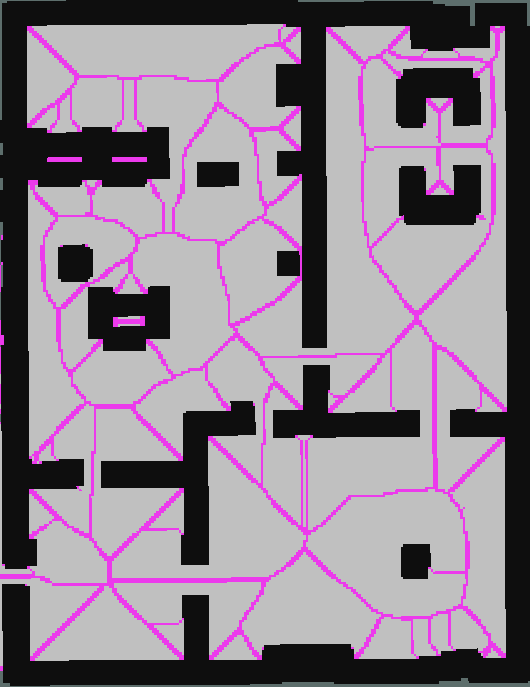
\includegraphics[width=\textwidth]{Figures/GVDFromGrid.png}
    \end{column}
  \end{columns}
\end{frame}

\begin{frame}\frametitle{El algoritmo \textit{Brushfire}}
  \begin{columns}
    \begin{column}{0.65\textwidth}
      \begin{algorithm}[H]
        \DontPrintSemicolon
        \KwData {Mapa de celdas de ocupación $M$}
        \KwResult{Distancias de cada celda al objeto más cercano}
        \;
        Fijar $d(p) = 0$ para toda celda $p$ en los obstáculos\;
        Fijar $d(p) = -1$ para toda celda $p$ en el espacio libre\;
        Crear una cola $Q$ y agregar toda $p$ en los obstáculos\;
        \While{$Q$ no esté vacía}
              {
                $x = $ desencolar de Q\;
                \ForAll{celdas $p$ vecinas de $x$}
                       {
                         \uIf{$d(p) == -1$}
                            {
                              Agregar $p$ a $Q$\;
                              Fijar $d(p) = x + d(p,x)$\;
                            }
                            \Else
                                {
                                  Fijar $d(p) = min(d(p), x+d(p,x))$
                                }
                       }
              }
        \caption{Brushfire}
        \end{algorithm}
    \end{column}
    \begin{column}{0.35\textwidth}
      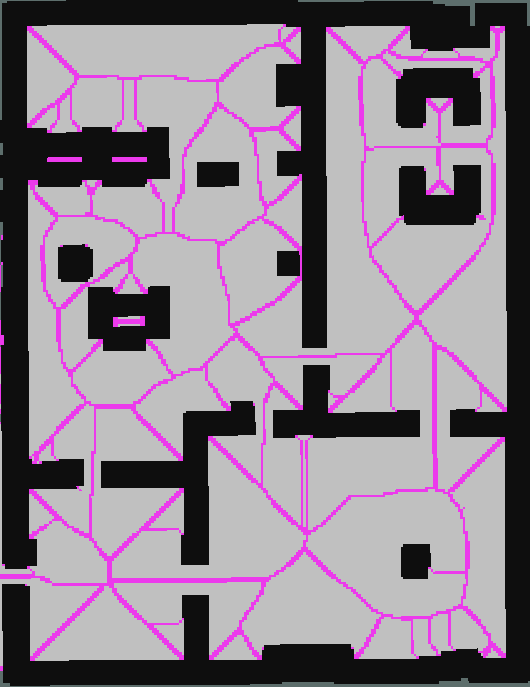
\includegraphics[width=\textwidth]{Figures/GVDFromGrid.png}
    \end{column}
  \end{columns}
\end{frame}


\begin{frame}[containsverbatim]\frametitle{Ejercicio 2 - Representación del ambiente}
  \begin{enumerate}
  \item Abra el archivo \texttt{catkin\_ws/src/students/scripts/assignment02a.py} e implemente el algoritmo de inflado de mapas (algoritmo \ref{alg:inflation}, diapositiva \ref{fr:inflation})
  \item Abra una terminal y corra la simulación con el comando (revise las instrucciones en el README del repositorio):
\begin{verbatim}
 roslaunch bring_up path_planning.launch
\end{verbatim}
  \item En otra terminal, corra el ejercicio 2a con el comando:
\begin{verbatim}
 rosrun students assignment02a.py _inflation_radius:=0.2
\end{verbatim}
  \item Obseve lo que sucede en el visualizador RViz.
  \item Detenga la práctica y ejecútela de nuevo con radios de inflado diferentes, por ejemplo:
\begin{verbatim}
 rosrun students assignment02a.py _inflation_radius:=0.3
\end{verbatim}
Observe qué sucede. ¿Qué pasa si el radio de inflado es muy grande o muy pequeño?
  \item En otra terminal, corra el algoritmo \textit{split and merge} con el comando:
\begin{verbatim}
 rosrun students assignment02b.py _dist:=0.01 _points:=3 _rho:=0.05 _theta:=0.05
\end{verbatim}
\item Detenga la detección de líneas y ejecútela nuevamente con diferentes parámetros de sintonización. Con la GUI, mueva el robot a diferentes puntos del mapa para verificar la correcta sintonización de dicho parámetros.
  \end{enumerate}
\end{frame}

\begin{frame}[containsverbatim]\frametitle{Ejercicio 2 - Representación del ambiente}
    \begin{enumerate}
    \setcounter{enumi}{7}
  \item En otra terminal, corra el algoritmo \textit{Brushfire} para obtener un Diagrama de Voronoi Generalizado a partir del mapa inflado (el ejercicio 02a debe estar corriendo):
\begin{verbatim}
 rosrun students assignment02c.py
\end{verbatim}

  \item Detenga el GVD y abra el archivo \texttt{catkin\_ws/src/students/scripts/assignment02c.py} y en las líneas 54 y 57 cambie la distancia Euclideana por distancia de Manhattan (revise los comentarios arriba de cada línea).
  \item Ejecute nuevamente la obtención del GVD y observe lo que sucede en el visualizador RViz
  \end{enumerate}
\end{frame}


\begin{frame}\frametitle{Planeación de rutas}
  La planeación de rutas consiste en encontrar una secuencia de puntos $q\in Q_{free}$ que permitan al robot moverse desde una configuración inicial $q_{start}$ hasta una configuración final $q_{goal}$.
  \begin{itemize}
  \item Una \textbf{ruta} es solo la secuencia de configuraciones para llegar a la meta.
  \item Cuando la secuencia de configuraciones se expresa en función del tiempo, entonces se tiene una \textbf{trayectoria}. 
  \end{itemize}
  En este curso solo vamos a hacer planeación de rutas, no de trayectorias (para navegación).\\
  Existen varios métodos para planear rutas. La mayoría de ellos se pueden agrupar en:
  \begin{itemize}
  \item Métodos basados en muestreo
  \item Métodos basados en grafos
  \end{itemize}
\end{frame}

\begin{frame}\frametitle{Métodos basados muestreo}
  Como su nombre lo indica, consisten en tomar muestras aleatorias del espacio libre. Si es posible llegar en línea recta de la configuración actual al punto muestrado, entonces se agrega a la ruta.
  Ejemplos:
  \begin{itemize}
  \item RRT (Rapidly-exploring Random Trees)
  \item RRT-Bidireccional
  \item RRT-Extendido
  \end{itemize}
\end{frame}

\begin{frame}\frametitle{\textit{Rapidly-exploring Random Trees}}
  Consiste en construir un árbol a partir de muestras aleatorias del espacio libre.
  \begin{columns}
    \begin{column}{0.4\textwidth}
      \begin{algorithm}[H]\small
        \KwData{Mapa, $q_{s} = $ Punto origen }
        \KwResult{Espacio explorado}
        Árbol[0] = $q_{s}$\;
        $k$ = 0\;
        \While{$k < k_{max}$ }
              {
                $q_{r}$ = ConfiguracionAleaoria()\;
                Extiende(Árbol, $q_{r}$)\;
                $k++$\;
              }
              \Return Árbol\;
              \caption{RRT}
      \end{algorithm}
    \end{column}
    \begin{column}{0.6\textwidth}
      \begin{figure}
        \centering
        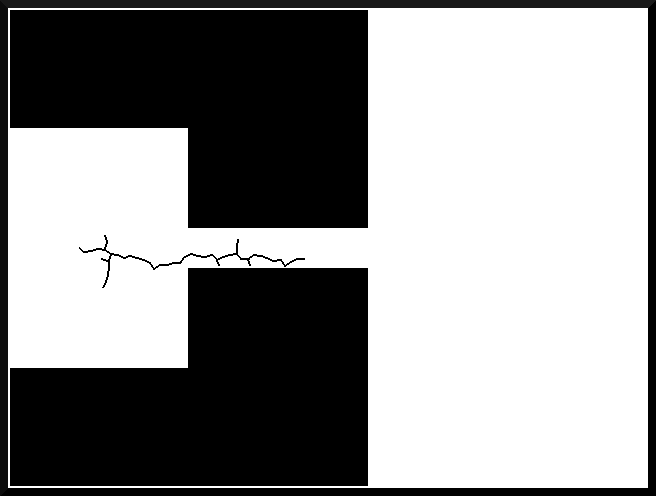
\includegraphics[width=0.45\textwidth]{Figures/RRTO010.png}
        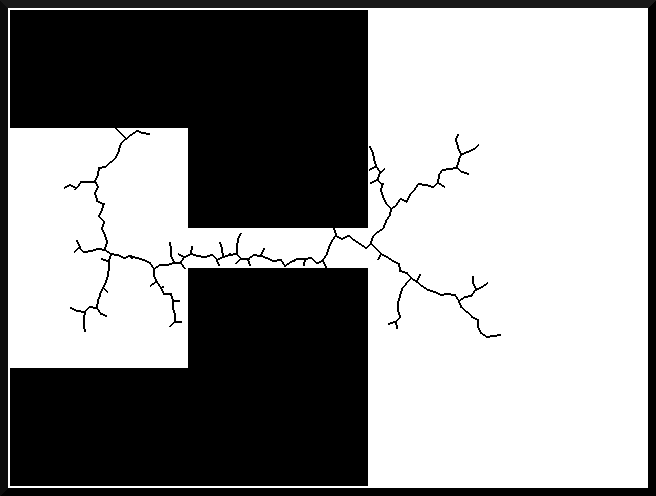
\includegraphics[width=0.45\textwidth]{Figures/RRTO0100.png}
        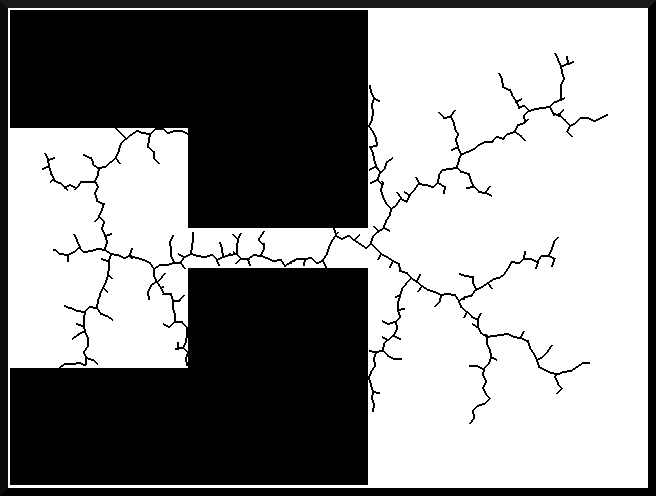
\includegraphics[width=0.45\textwidth]{Figures/RRTO0300.png}
      \end{figure}
    \end{column}
  \end{columns}
\end{frame}

\begin{frame}\frametitle{Métodos basados en grafos}
  Estos métodos consideran el ambiente como un grafo. En el caso de celdas de ocupación, cada celda libre es un nodo que está conectado con las celdas vecinas que también estén libres. Los pasos generales de este tipo de algorimos se pueden resumir en:
  \[\]
  \begin{algorithm}[H]
    \footnotesize
    \DontPrintSemicolon
    \KwData {Mapa $M$ de celdas de ocupación, configuración inicial $q_{start}$, configuración meta $q_{goal}$}
    \KwResult{Ruta $P=[q_{start},q_1, q_2, \dots , q_{goal}]$}
    Obtener los nodos $n_s$ y $n_g$ correspondientes a $q_{start}$ y $q_{goal}$\;
    Lista abierta $OL = \emptyset$ y lista cerrada $CL = \emptyset$\;
    Agregar $n_s$ a $OL$\;
    Nodo actual $n_c = n_s$\;
    \While{$OL\neq \emptyset$ y $n_c\neq n_g$}
    {
      Seleccionar $n_c$ de $OL$ \textbf{bajo algún criterio}\;
      Agregar $n_c$ a $CL$\;
      Expandir $n_c$\;
      Agregar a $OL$ los vecinos de $n_c$ que no estén ya en $OL$ ni en $CL$\;
    }
    \If{$n_c\neq n_g$}{Anunciar Falla}
    Obtener la configuración $q_i$ para cada nodo $n_i$ de la ruta\;
  \end{algorithm}
\end{frame}

\begin{frame}\frametitle{Métodos basados en grafos}
  El criterio para seleccinar el siguiente nodo a expandir $n_c$ de la lista abierta, determina el tipo de algoritmo:
  \begin{itemize}
  \item Criterio FIFO: Búsqueda a lo ancho BFS (la lista abierta es una cola)
  \item Criterio LIFO:  Búsqueda en profundidad DFS (la lista abierta es una pila)
  \item Menor valor $g$: Dijkstra (la lista abierta es una cola con prioridad)
  \item Menor valor $f$: A* (la lista abierta es una cola con prioridad)
  \end{itemize}
  Si el costo $g$ para ir de una celda a otra es siempre 1, entonces Dijkstra es equivalente a BFS. \\
  A* y Dijkstra siempre calculan la misma ruta pero A* lo hace más rápido. 
\end{frame}

\begin{frame}\frametitle{Mapas de costo}
  \begin{itemize}
  \item Los métodos como Dijkstra y A* minimizan una función de costo. Esta función podría ser distancia, tiempo de recorrido, número de vuelta, energía gastada, entre otras.
  \item En este curso se empleará como costo una combinación de distancia recorrida más peligro de colisión (cercanía a los obstáculos).
  \item De este modo, las rutas serán un equilibrio entre rutas cortas y rutas seguras.
  \end{itemize}
  \begin{figure}
    \centering
    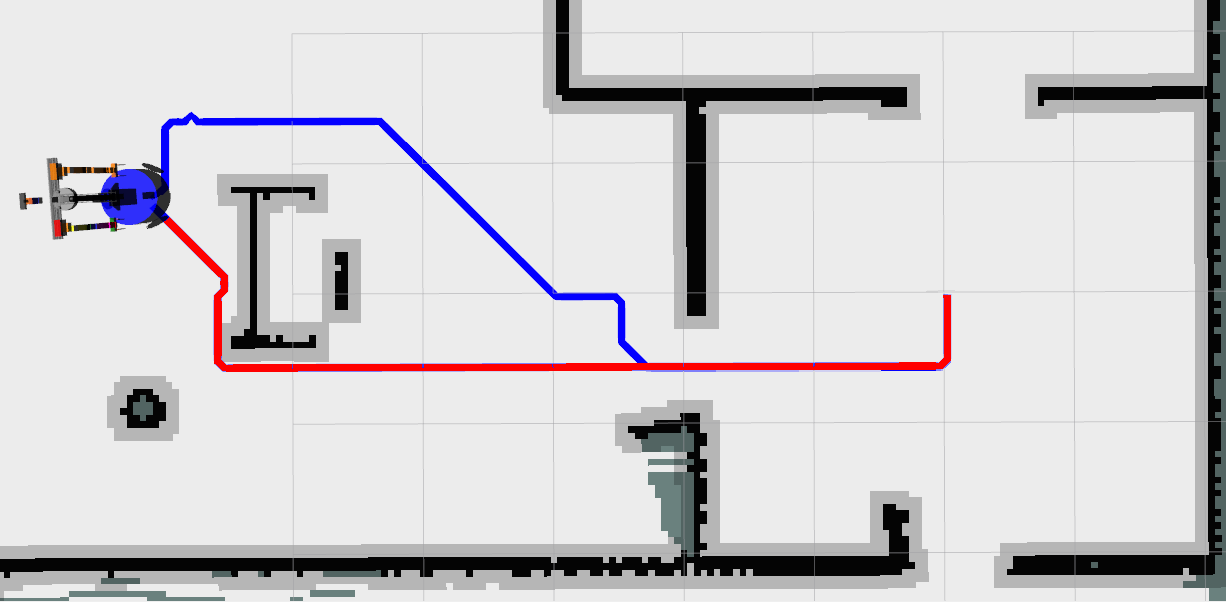
\includegraphics[width=0.5\textwidth]{Figures/AStarComparison.png}
  \end{figure}
\end{frame}

\begin{frame}\frametitle{Mapas de costo}
  \begin{itemize}
  \item Se utilizará como costo una función de \textit{cercanía}.
  \item Se calcula de forma similar al algoritmo Brushfire, pero la función decrece conforme nos alejamos de los objetos. 
  \end{itemize}
  \begin{columns}
    \begin{column}{0.6\textwidth}
      \begin{algorithm}[H]
        \footnotesize
        \DontPrintSemicolon
        \KwData {\;
          Mapa $M$ de celdas de ocupación\;
          Radio de costo $r_c$
        }
        \KwResult{Mapa de costo $M_c$}
        \;
        $M_c = $ Copia de $M$\;
        \ForEach{$i\in [0,\dots,rows)$}
          {
            \ForEach{$j\in [0,\dots,cols)$}
              {
                //Si está ocupada, calcular el costo de $r_c$ celdas alrededor.\;
                \If{$M[i,j] == 100$ }
                   {
                     \ForEach{$k_1\in [-r_c,\dots,r_c]$}
                             {
                               \ForEach{$k_2\in [-r_c,\dots,r_c]$}
                                       {
                                         $C = r_c - max(|k1|,|k2|) + 1$\;
			                 $M_c[i+k1,j+k2] = max(C, M_c[i+k1,j+k2]$\;
                                       }
                             }
                   }    
              }
            }
            \caption{Mapa de costo}
      \end{algorithm}
    \end{column}
    \begin{column}{0.4\textwidth}
      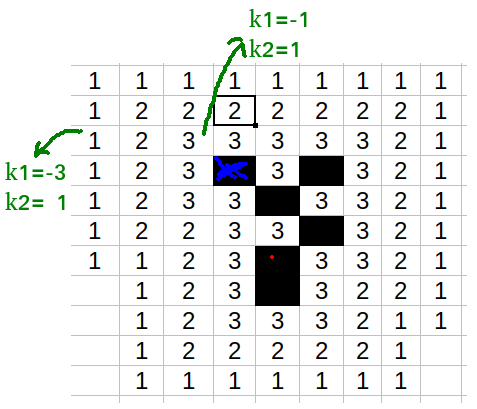
\includegraphics[width=0.95\textwidth]{Figures/CostMap.png}
    \end{column}
  \end{columns}
\end{frame}


%%%%%%%%%%%%%%%%%%%
%%% 2023-09-05 %%%%
%%%%%%%%%%%%%%%%%%%
\section{El algoritmo A* (2023-09-05)}

\begin{frame}\frametitle{El algoritmo A*}
  \begin{itemize}
  \item Es un algoritmo completo, es decir, si la ruta existe, seguro la encontrará, y si no existe, lo indicará en tiempo finito.
  \item Al igual que Dijkstra, A* encuentra una ruta que minimiza una función de costo, es decir, es un algoritmo óptimo.
  \item Es un algoritmo del tipo de búsqueda informada, es decir, utiliza información sobre el estimado del costo restante para llegar a la meta para priorizar la expansión de ciertos nodos. 
  \item El nodo a expandir se selecciona de acuerdo con la función:
    \[f(n) = g(n) + h(n)\]
    donde
    \begin{itemize}
    \item $g(n)$ es el costo acumulado del nodo $n$
    \item $h(n)$ es una función heurística que \textbf{subestima} el costo de llegar del nodo $n$ al nodo meta $n_g$. 
    \end{itemize}
  \item Se tienen los siguientes conjuntos importantes:
    \begin{itemize}
    \item Lista abierta: conjunto de todos los nodos en la frontera (visitados pero no conocidos). Es una cola con prioridad donde los elementos son los nodos y la prioridad es el valor $f(n)$.
    \item Lista cerrada: conjunto de nodos para los cuales se ha calculado una ruta óptima. 
    \end{itemize}
    \item A cada nodo se asocia un valor $g(n)$, un valor $f(n)$ y un nodo padre $p(n)$. 
  \end{itemize}
\end{frame}

\begin{frame}\frametitle{El algoritmo A*}
    \begin{algorithm}[H]
    \footnotesize
    \DontPrintSemicolon
    \KwData {Mapa $M$, nodo inicial $n_s$ con configuración $q_{s}$, nodo meta $n_g$ con configuración $q_{g}$}
    \KwResult{Ruta óptima $P=[q_{s},q_1, q_2, \dots , q_{g}]$}
    Lista abierta $OL = \emptyset$ y lista cerrada $CL = \emptyset$\;
    Fijar $f(n_{s}) = 0$, $g(n_{s}) = 0$ y $prev(n_{s}) = NULL$\;
    Agregar $n_s$ a $OL$ y fijar nodo actual $n_c = n_s$\;
    \While{$OL\neq \emptyset$ y $n_c\neq n_g$}
    {
      Remover de $OL$ el nodo $n_c$ con el menor valor $f$ y agregar $n_c$ a $CL$\;
      \ForAll{$n$ vecino de $n_c$}
             {
               $g = g(n_c) + costo(n_c, n)$\;
               \If{$g < g(n)$}
                  {
                    $g(n) = g$\;
                    $f(n) = h(n) + g(n)$\;
                    $prev(n) = n_c$\;
                  }
             }
      Agregar a $OL$ los vecinos de $n_c$ que no estén ya en $OL$ ni en $CL$\;
    }
    \If{$n_c\neq n_g$}{Anunciar Falla}
    \While{$n_c \neq NULL$}
          {
            Insertar al inicio de la ruta $P$ la configuración correspondiente al nodo $n_c$\;
            $n_c = prev(n_c)$
          }
    Devolver ruta óptima $P$
  \end{algorithm}
\end{frame}

\begin{frame}\frametitle{El algoritmo A*}
  \begin{itemize}
  \item La función de costo será el número de celdas más el mapa de costo obtenido anteriormente.
  \item Puesto que el mapa está compuesto por celdas de ocupación, los nodos vecinos se pueden obtener usando conectividad 4 o conectividad 8.
  \item Si se utiliza conectividad 4, la distancia de Manhattan es una buena heurística.
  \item Si se utiliza conectividad 8, se debe usar la distancia Euclideana.
  \item La lista abierta se puede implementar con una \textit{Heap}, de este modo, la inserción de los nodos $n$ se puede hacer en tiempo logarítmico y la selección del nodo con menor $f$ se hace en tiempo constante.
  \item La obtención de las coordenadas $(x,y)$ a partir de los nodos $n$ se puede hacer con:
    \begin{eqnarray*}
      x &=& (c)\delta + M_{ox}\\
      y &=& (r)\delta + M_{oy}
    \end{eqnarray*}
  \item La obtención del renglón-columna $(r,c)$ del nodo $n$ a partir de $(x,y)$, se puede obtener con:
    \begin{eqnarray*}
      r &=& int((y - M_{oy})/\delta)\\
      c &=& int((x - M_{ox})/\delta)
    \end{eqnarray*}
    donde
    \begin{itemize}
    \item $(M_{ox}, M_{oy})$ es el origen del mapa, es decir, las coordenadas cartesianas de la celda (0,0).
    \item $\delta$ es la resolución, es decir, el tamaño de cada celda.
    \item La función $int()$ convierte a entero el argumento. 
    \end{itemize}
    \item Todos estos valores están en los metadatos del mapa. 
  \end{itemize}
\end{frame}

\begin{frame}\frametitle{El algoritmo A*}
  Ejemplo: ¿Cuál es la ruta óptima del nodo A al nodo Z?
  \begin{figure}
    \centering
    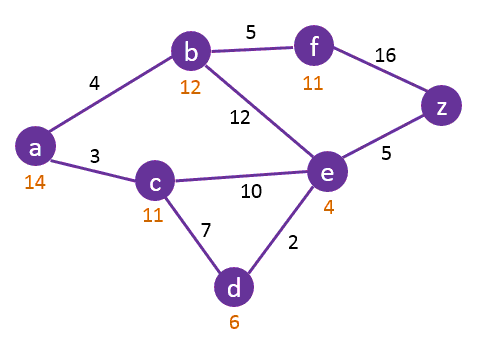
\includegraphics[width=0.5\textwidth]{Figures/AStarExample.png}
  \end{figure}
\end{frame}

\begin{frame}\frametitle{El algoritmo A*}
  \begin{table}
    \begin{tabular}{cccc}
      Paso & Nodo actual & Lista Cerrada & Lista abierta\\
      \hline
      0   & NULL & $\emptyset$          & \{A\}      \\
      1   & A    & \{A\}                & \{B, C\}   \\
      2   & C    & \{A, C\}             & \{B, D, E\}\\
      3   & B    & \{A, C, B\}          & \{D, E, F\}\\
      4   & D    & \{A, C, B, D\}       & \{E, F\}   \\
      5   & $E$  & \{A, C, B, D, E\}    & \{F, Z\}   \\
      6   & $Z$  & \{A, C, B, D, E, Z\} & \{F \}     \\
    \end{tabular}
  \end{table}
  \begin{table}
    \footnotesize
    \begin{tabular}{ccccccc}
      A & B & C & D & E & F & Z \\
      g,f,p & g,f,p & g,f,p & g,f,p & g,f,p & g,f,p & g,f,p\\
      \hline
      0,0,NULL & $\infty,\infty$,NULL & $\infty,\infty$,NULL & $\infty,\infty$,NULL & $\infty,\infty$,NULL & $\infty,\infty$,NULL & $\infty,\infty$,NULL\\
      0,0,NULL & 4, 16, A             & 3, 14, A             & $\infty,\infty$,NULL & $\infty,\infty$,NULL & $\infty,\infty$,NULL & $\infty,\infty$,NULL\\
      0,0,NULL & 4, 16, A             & 3, 14, A             & 10, 16, C            & 13, 17, C            & $\infty,\infty$,NULL & $\infty,\infty$,NULL\\
      0,0,NULL & 4, 16, A             & 3, 14, A             & 10, 16, C            & 13, 17, C            & 9, 20, B             & $\infty,\infty$,NULL\\
      0,0,NULL & 4, 16, A             & 3, 14, A             & 10, 16, C            & \textbf{12, 16, D}   & 9, 20, B             & $\infty,\infty$,NULL\\
      0,0,NULL & 4, 16, A             & 3, 14, A             & 10, 16, C            &         12, 16, D    & 9, 20, B             & 17, 17, E           \\
      0,0,NULL & 4, 16, A             & 3, 14, A             & 10, 16, C            &         12, 16, D    & 9, 20, B             & 17, 17, E           \\
    \end{tabular}
  \end{table}
\end{frame}

\begin{frame}[containsverbatim]\frametitle{Ejercicio 03 - Planeación de rutas}
  Realice lo siguiente:
  \begin{enumerate}
     \item Abra el archivo \texttt{catkin\_ws/src/students/scripts/assignment03a.py} y agregue el siguiente código en la línea 45:
  \begin{lstlisting}[language=Python,firstnumber=45]
for i in range(height):
    for j in range(width):
        if static_map[i,j] > 50:
            for k1 in range(-cost_radius, cost_radius+1):
                for k2 in range(-cost_radius, cost_radius+1):
                    cost = cost_radius - max(abs(k1),abs(k2)) + 1
                    cost_map[i+k1,j+k2] = max(cost, cost_map[i+k1,j+k2])
                  \end{lstlisting}
  \item Corra el simulador con el comando
\begin{verbatim}
    roslaunch bring_up path_planning.launch
\end{verbatim}                  
  \item Corra los nodos de inflado de mapas, mapa de costo y A*, para ello, en tres terminales diferentes, corra los comandos:
\begin{verbatim}
    rosrun students assignment02a.py _inflation_radius:=0.25
    rosrun students assignment03a.py _cost_radius:=0.3
    rosrun students assignment03b.py
\end{verbatim}
  \end{enumerate}
\end{frame}

\begin{frame}\frametitle{Ejercicio 03 - Planeación de rutas}
  \begin{enumerate}
    \setcounter{enumi}{3}
  \item Calcule una ruta utilizando los campos Start Pose y Goal Pose de la GUI:
    \begin{figure}
      \centering
      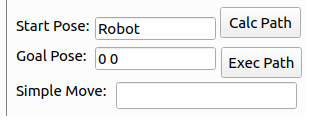
\includegraphics[width=0.35\textwidth]{Figures/GUIPathPlanning.png}
    \end{figure}
  \item Detenga y ejecute de nuevo el inflado de mapas con radios entre 0.1 y 0.5 m y vea qué sucede con el cálculo de rutas.
  \item Detenga y ejecute de nuevo el cálculo del mapa de costo con radios de entre 0.05 y 0.5 m y vea qué sucede con las rutas. 
  \item En el archivo \texttt{assignment03b.py}, cambie la función de distancia de Manhattan por distancia Euclideana, y cambie la conectividad 4 por conectividad 8 (líneas 44, 68 y 69) y vea qué sucede.
  \item Modifique el código para que $h$ sea siempre cero (línea 69) y vea qué sucede con el número de pasos. Pruebe con varias rutas. 
  \end{enumerate}
\end{frame}

\begin{frame}\frametitle{Seguimiento de rutas}
  Hasta el momento ya se tiene una representación del ambiente y una forma de planear rutas. Ahora falta diseñar las leyes de control que hagan que el robot se mueva por la ruta calculada. Este control se hará bajo los siguientes supuestos:
  \begin{itemize}
  \item Se conoce la posición del robot (más adelante se abodará el problema de la localización)
  \item El modelo cinemático es suficiente para modelar el movimiento del robot 
  \item Las dinámicas no modeladas (parte eléctrica y mecánica de los motores) son lo suficientemente rápidas para poder despreciarse
  \end{itemize}
\end{frame}

\begin{frame}\frametitle{Modelo cinemático}
  Considere la base móvil omnidireccional de la figura con configuración $q=(x,y,\theta)$.
  \begin{columns}
    \begin{column}{0.5\textwidth}
      \begin{figure}
        \centering
        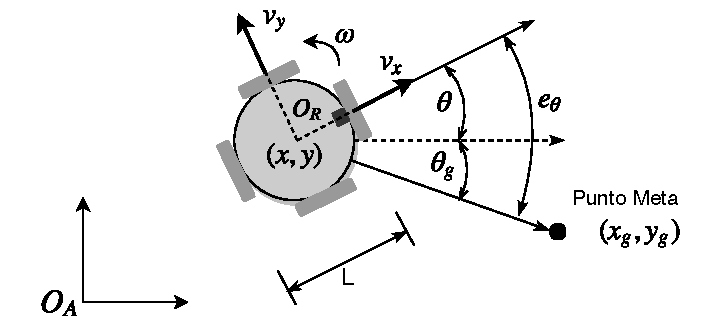
\includegraphics[width=\textwidth]{Figures/GoalPose.pdf}
      \end{figure}
    \end{column}
    \begin{column}{0.5\textwidth}
      El modelo cinemático está dado por
      \begin{eqnarray*} 
        \dot{x} &=& v_x\cos\theta - v_y\sin\theta\label{eq:Kinematic1}\\         
        \dot{y} &=& v_x\sin\theta + v_y\cos\theta\\ 
        \dot{\theta} &=& \omega,\label{eq:Kinematic3}
      \end{eqnarray*}
    \end{column}
  \end{columns}
  \[\]
  \begin{itemize}
  \item $(v_x, v_y, \omega)$ se consideran como señales de control
  \item Corresponden a las velocidades lineales frontal y lateral, y la velocidad angular, con respecto al robot.
  \item La forma de convertir $(v_x, v_y, \omega)$ a velocidades de cada motor varía dependiendo del número de motores y de su posición. 
  \end{itemize}
\end{frame}

\begin{frame}\frametitle{Base omnidireccional de 4 ruedas}
  Dada una base omnidireccional con las ruedas colocadas como se muestra en la figura, las velocidades de cada llanta se pueden obtener como:
  \[\]
  \begin{columns}
    \begin{column}{0.4\textwidth}
      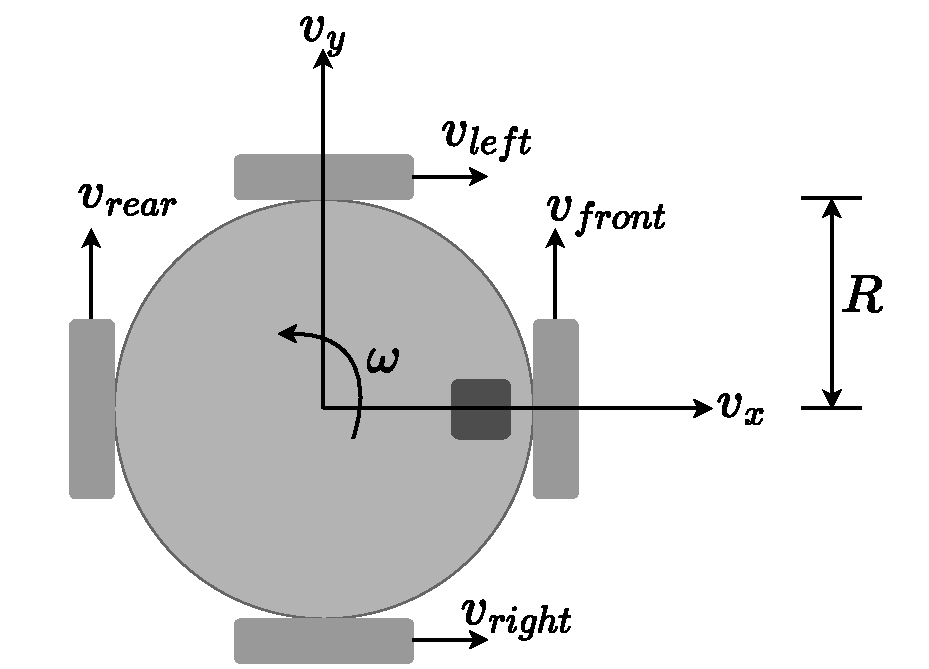
\includegraphics[width=\textwidth]{Figures/Omnidirectional4wheels.pdf}
    \end{column}
    \begin{column}{0.6\textwidth}
      \[\left[\begin{array}{c}
          v_{left}\\v_{right}\\v_{front}\\v_{rear}
              \end{array}\right] =
        \left[\begin{array}{ccc}
                    1 & 0 & -R\\
                    1 & 0 & +R\\
                    0 & 1 & +R\\
                    0 & 1 & -R
        \end{array}\right]
        \left[\begin{array}{c}
           v_{x}\\v_{y}\\ \omega 
        \end{array}\right]
        \]
  \begin{itemize}
  \item Las velocidades de las llantas son lineales.
  \item Para obtener las velocidades angulares, basta con dividir entre el radio de las llantas.
  \end{itemize}
\end{column}
\end{columns}
\[\]
\begin{itemize}
\item Como se puede observar, la matriz anterior no tiene inversa.
\item Se tienen cuatro velocidades de llantas en función de tres variables $(v_x,v_y, \omega)$
\item Esto significa que dadas tres velocidades de llantas, \textbf{la cuarta no puede ser cualquier valor}
\end{itemize}
\end{frame}

\begin{frame}\frametitle{Base omnidireccional de 3 ruedas}
  \begin{itemize}
  \item La base de 4 ruedas omnidireccionales tiene la ventaja de tener mejor tracción y de lograr movimientos rectos más fácilmente.
  \item Tiene la desventaja de que las velocidades pueden indeterminarse si no están bien calculadas.
  \item Una base omnidireccional también puede lograrse con 3 ruedas:
  \end{itemize}
  \begin{columns}
    \begin{column}{0.4\textwidth}
      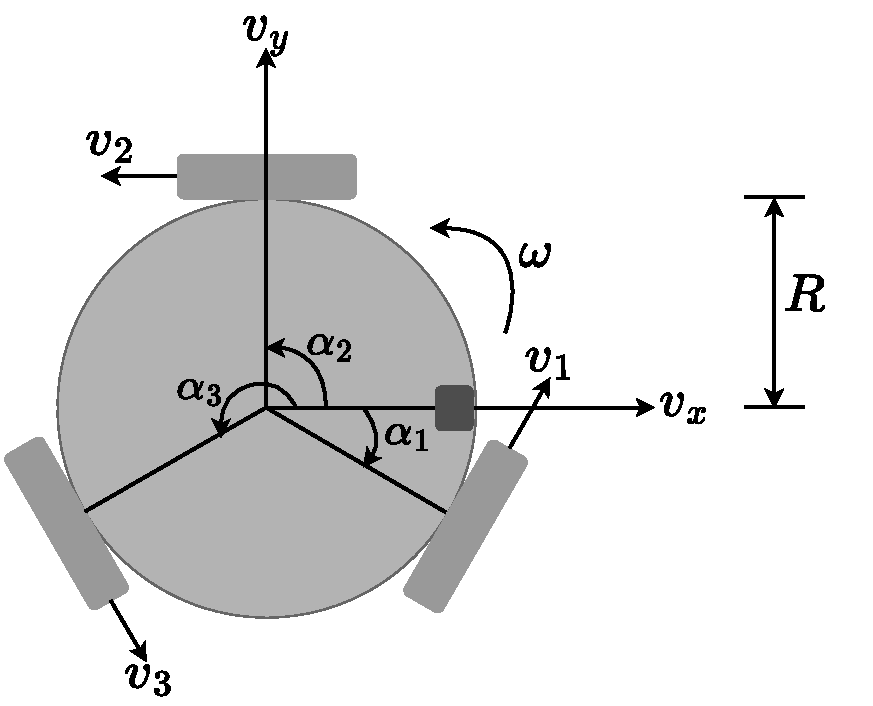
\includegraphics[width=\textwidth]{Figures/Omnidirectional3wheels.pdf}
    \end{column}
    \begin{column}{0.6\textwidth}
      \[\left[\begin{array}{c}
          v_1\\v_2\\v_3
              \end{array}\right] =
        \left[\begin{array}{ccc}
                    -\sin\alpha_1 & \cos\alpha_1 & R\\
                    -\sin\alpha_2 & \cos\alpha_2 & R\\
                    -\sin\alpha_3 & \cos\alpha_3 & R\\
        \end{array}\right]
        \left[\begin{array}{c}
           v_{x}\\v_{y}\\ \omega 
        \end{array}\right]
        \]
\end{column}
\end{columns}
\end{frame}

\begin{frame}\frametitle{Base diferencial}
  \begin{itemize}
  \item Con una base diferencial ya no se tiene movimiento omnidireccional, es decir, se tiene movimiento no holonómico.
  \item El robot ya solo puede tener velocidad frontal $v_x$ pero no velocidad lateral $v_y$.
  \end{itemize}
  \begin{columns}
    \begin{column}{0.4\textwidth}
      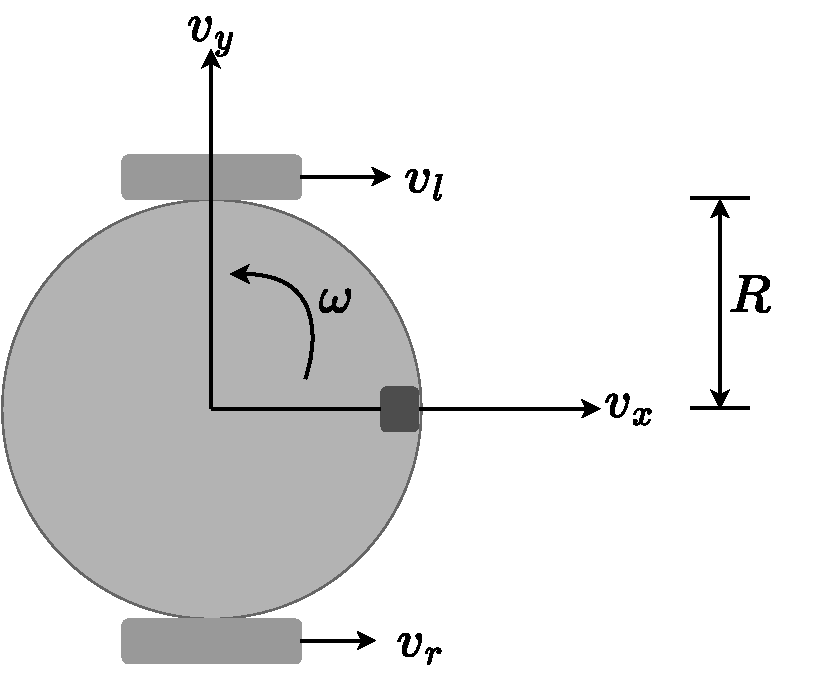
\includegraphics[width=\textwidth]{Figures/DifferentialBase.pdf}
    \end{column}
    \begin{column}{0.6\textwidth}
      \begin{eqnarray*}
        v_l &=& v_x - R\omega\\
        v_r &=& v_x + R\omega
      \end{eqnarray*}
    \end{column}
  \end{columns}
  Esta es la configuración más fácil de lograr debido a la simplicidad del hardware necesario. 
\end{frame}

\begin{frame}\frametitle{Base \textit{Ackermann}}
  
\end{frame}

\begin{frame}\frametitle{Control de posición}
  \begin{itemize}
  \item Las leyes de control se diseñarán considerando una base diferencial
  \item Es mejor mover al robot así, pues lo sensores están generalmente al frente
  \end{itemize}
  Si se quiere alcanzar el punto meta $(x_g, y_g)$, las siguientes leyes de control siguientes permiten alcanzar dicho punto meta:
  \begin{eqnarray*}
  v_x    &=& v_{max}e^{-\frac{e_{\theta}^{2}}{\alpha}}\label{eq:Control11}\\
  \omega &=& \omega_{max}\left(\frac{2}{1+e^{-\frac{e_{\theta}}{\beta}}}-1\right)\label{eq:Control12}
  \end{eqnarray*}
  con
  \[e_{\theta} = \atantwo\left(y_g - y, x_g - x\right) - \theta\]
  El error de ángulo $e_\theta$ debe estar siempre en el intervalo $(-\pi, \pi]$. Si la diferencia resulta en un valor fuera de este ángulo, se puede acotar mediante:
  \[e_\theta \leftarrow \left(e_\theta + \pi\right)\% (2\pi) - \pi\]
  donde \% denota el operador módulo (residuo). 
\end{frame}

\begin{frame}\frametitle{Control de posición}
  \begin{itemize}
  \item $v_{max}$ y $\omega_{max}$ son las velocidades linear y angular máximas y dependen de las capacidades físicas del robot.
  \item $\alpha$ y $\beta$ determinan qué tan rápido varían dichas velocidades cuando cambia el error de ángulo.
  \item En general, valores pequeños de $\alpha$ y $\beta$ logran que el robot alcance el punto meta casi en línea recta, sin embargo, valores muy pequeños pueden producir oscilaciones.
  \item Valores grandes de $\alpha$ y $\beta$ producen un movimiento más suave pero pueden hacer que el robot describa curvas muy extensas. 
  \end{itemize}
  \begin{figure}
    \centering
    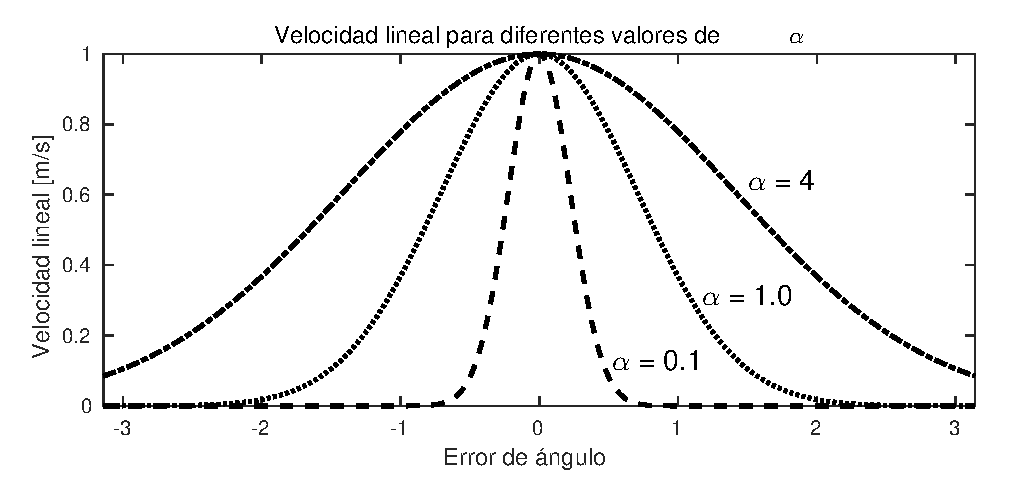
\includegraphics[width=0.45\textwidth]{Figures/LinearSpeed.eps}
    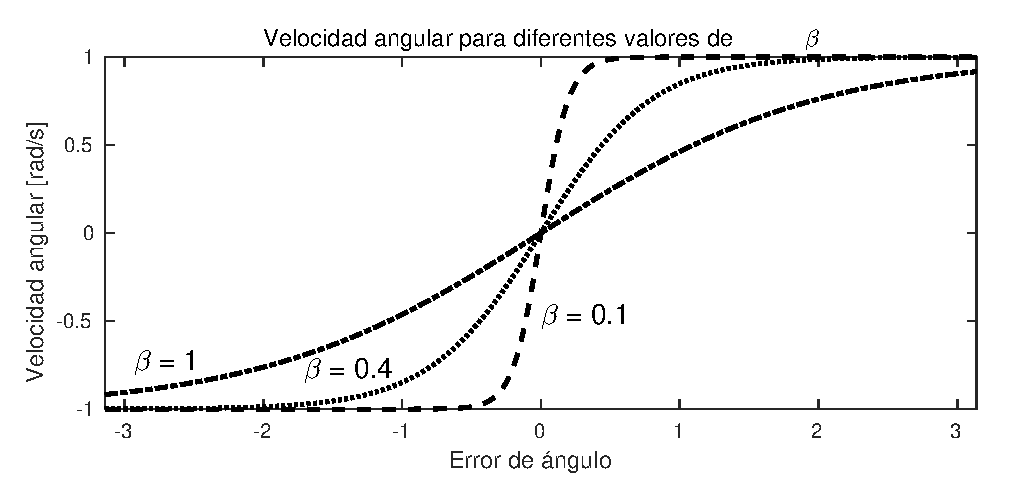
\includegraphics[width=0.45\textwidth]{Figures/AngularSpeed.eps}
  \end{figure}
\end{frame}

\begin{frame}\frametitle{Control de base omnidireccional}
\end{frame}

\begin{frame}\frametitle{Seguimiento de rutas}
  \begin{itemize}
  \item Hasta el momento se ha planteado cómo alcanzar una posición, pero, ¿para una ruta?
  \item Las rutas son secuencias de puntos. Esta secuencia se podría parametrizar con respecto al tiempo para tener una trayectoria, sin embargo esto resulta muy complicado debido a la complejidad de las rutas.
  \item Una solución más sencilla es aplicar el control de posición para cada punto hasta recorrer toda la ruta.
  \item Las leyes de control solo dependen de $e_\theta$ por lo que el robot no desacelera al acercarse a la meta, provocando fuertes oscilaciones.
  \item Una forma de resolver este problema es ejecutar la ley de control sólo si la distancia al punto meta 

    \[d=\sqrt{(x_g - x_r)^2 + (y_g - y_r)^2}\] 
    
    es mayor que una tolerancia $\epsilon$.
  \item En este caso, el robot se detendrá abruptamente cuando el error de distancia sea menor que $\epsilon$, lo cual tampoco es deseable
  \item Una forma fácil de hacer que el robot acelere y desacelere, o en general, obtener un perfil de velocidad, es mediante el uso de una máquina de estados
    
  \end{itemize}
\end{frame}

\begin{frame}\frametitle{Perfil de velocidad}
  \begin{columns}
    \begin{column}{0.43\textwidth}
      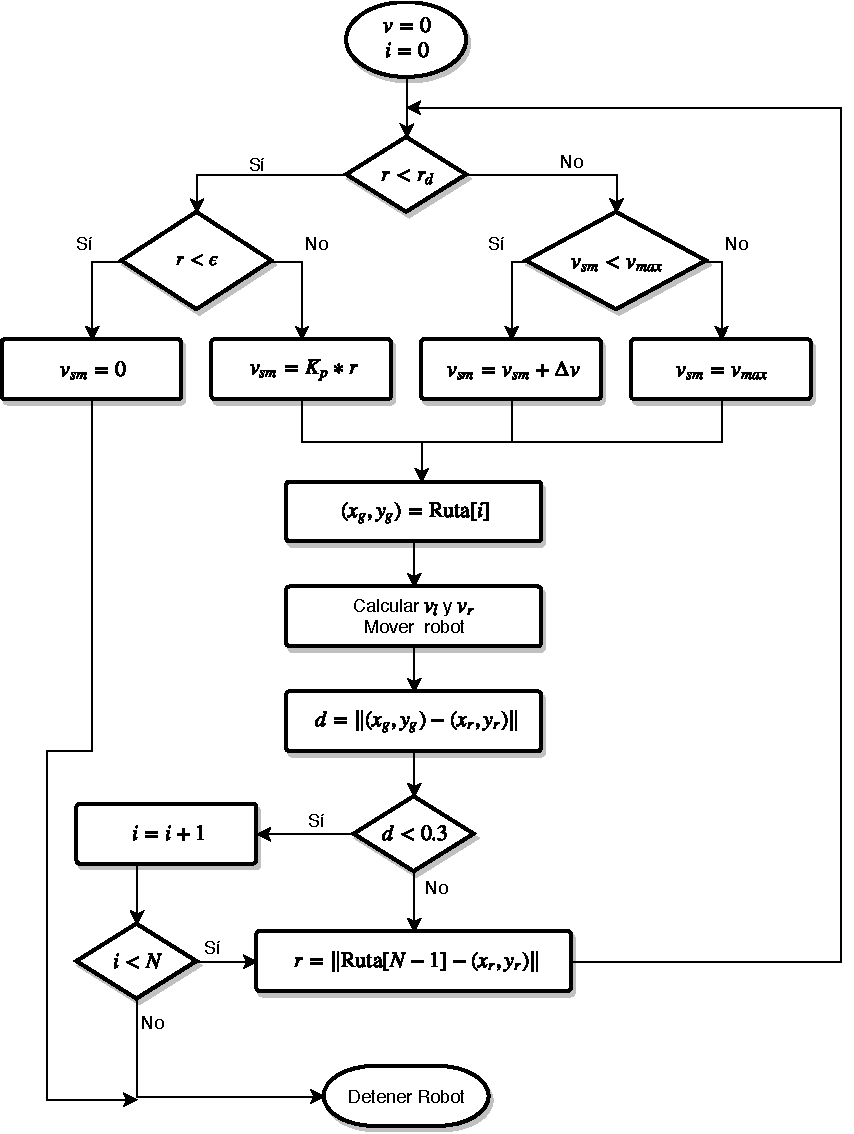
\includegraphics[width=\textwidth]{Figures/AFSM.pdf}
    \end{column}
    \begin{column}{0.5\textwidth}
      Considere una máquina de estados que calcule $v_{max}$ en el control. Sea $v_{sm}$ la nueva velocidad lineal máxima, de modo que ahora se tiene:
      \begin{eqnarray*}
        v      &=& v_{sm}e^{-\frac{e_{\theta}^{2}}{\alpha}}\label{eq:NewControl1}\\
        \omega &=& \omega_{max}\left(\frac{2}{1+e^{-\frac{e_{\theta}}{\beta}}}-1\right)\label{eq:NewControl2}
      \end{eqnarray*}
      con
      \begin{itemize}
      \item $r$: Distancia a la meta global
      \item $\epsilon$: Distancia a la que se considera que el robot alcanzó la meta global
      \item $r_d$: Distancia a la meta global para desacelerar
      \item $\Delta v$: Aceleración 
      \end{itemize}
    \end{column}
  \end{columns}
\end{frame}

\begin{frame}\frametitle{Perfil de velocidad}
  La siguiente figura muestra un ejemplo de una ruta y las velocidades lineales generadas usando solo las leyes de control (izquierda) y usando la máquina de estados para un perfil de velocidad (derecha). 
  \begin{figure}
    \centering
    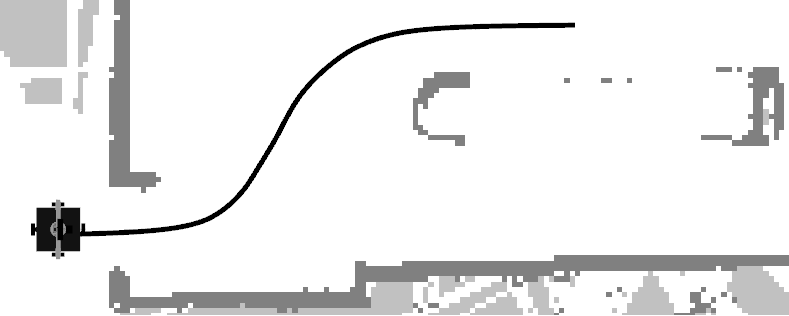
\includegraphics[width=0.45\textwidth]{Figures/SpeedProfilePath.png}
  \end{figure}
  \begin{figure}
    \centering
    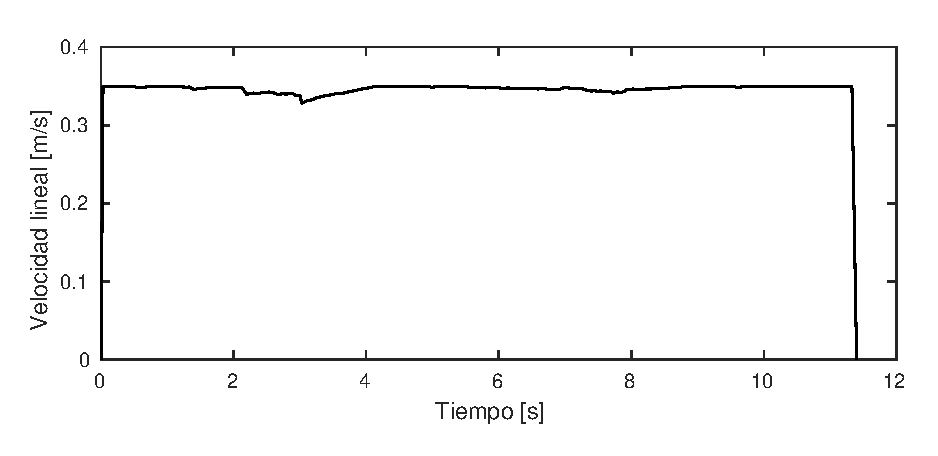
\includegraphics[width=0.45\textwidth]{Figures/SpeedWithoutProfile.eps}
    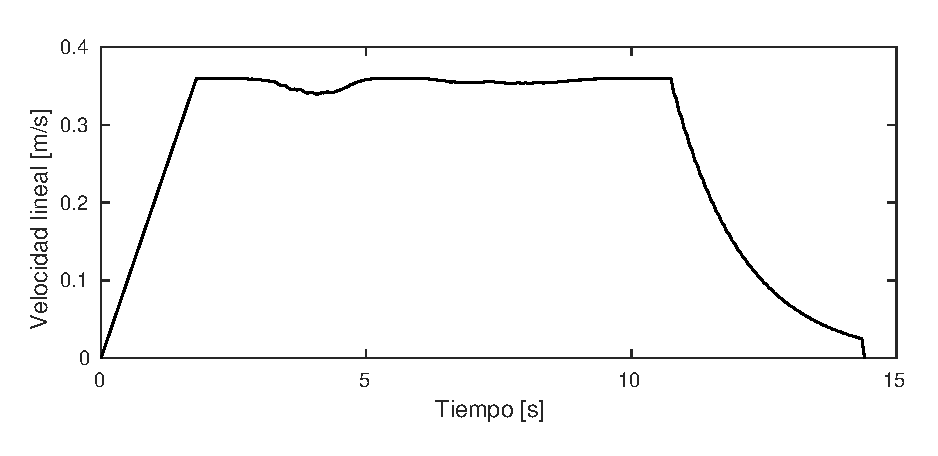
\includegraphics[width=0.45\textwidth]{Figures/SpeedWithProfile.eps}
  \end{figure}
\end{frame}

\begin{frame}[containsverbatim]\frametitle{Ejercicio 04 - Seguimiento de rutas}
Realice lo siguiente:
  \begin{enumerate}
  \item Abra el archivo \texttt{catkin\_ws/src/students/scripts/assignment05.py} e implemente las leyes de control para calcular $v$ y $\omega$ dentro de la función \texttt{calculate\_speeds}. Siga las instrucciones de los comentarios del código. 
  \item Ejecute la simulación igual que en los ejercicios anteriores. 
  \item Ejecute el inflado de obstáculos, mapa de costo, algoritmo A* y seguimiento de rutas (\texttt{assignment02a.py, assignment03a.py, assignment03b.py} y \texttt{assignment04.py})
  \item Con el botón \textit{2D Nav Goal} del visualizador \textit{RViz}, selecccione un punto meta en el mapa y observe qué sucede. 
  \item Pruebe con diferentes valores de $\alpha$ y $\beta$ hasta obtener un movimiento satisfactorio. 
  \end{enumerate}
\end{frame}


\begin{frame}\frametitle{Suavizado de rutas}
  \begin{itemize}
  \item Puesto que las rutas se calcularon a partir de celdas de ocupación, están compuestas de esquinas.
  \item La esquinas no son deseables, pues suelen generar cambios bruscos en las señales de control.
  \item La ruta verde de la imagen es una muestra de una ruta calculada por A*.
  \item Es preferible una ruta como la azul. 
  \end{itemize}
  \begin{figure}
    \centering
    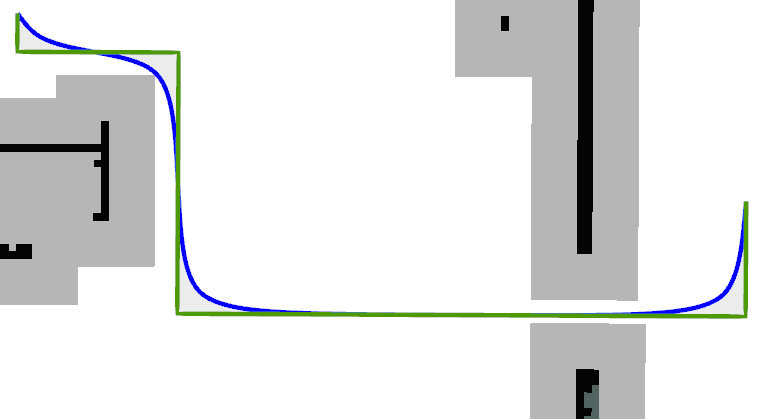
\includegraphics[height=0.45\textheight]{Figures/PathSmoothingExample.png}
  \end{figure}
  Existen varias formas de suavizar la ruta generada:
  \begin{itemize}
  \item Splines
  \item Descenso del gradiente
  \end{itemize}
\end{frame}

\begin{frame}\frametitle{Suavizado mediante splines}
  \begin{itemize}
  \item Un \textit{spline} es una función definida a tramos por polinomios.
  \item La forma más común son los splines de tercer grado o \textit{cubic splines}
  \item Se ajusta un polinomio de tercer grado por cada par de puntos
  \item La derivada al final de un tramo debe ser igual a la derivada al inicio del siguiente tramo.
  \item Aplicando estas condiciones para cada par 
  \end{itemize}
  
\end{frame}


\begin{frame}\frametitle{Suavizado mediante descenso del gradiente}
  Otra forma de suavizar la ruta es planteando una función de costo y encontrando el mínimo. Los puntos negros representan la ruta de A* compuesta por los puntos $Q=\{q_0, q_1, \dots, q_n\}$ y los puntos azules representan una ruta suave $P=\{p_0, p_1,\dots, p_n\}$.
  \begin{columns}
    \begin{column}{0.5\textwidth}
      \begin{figure}
        \centering
        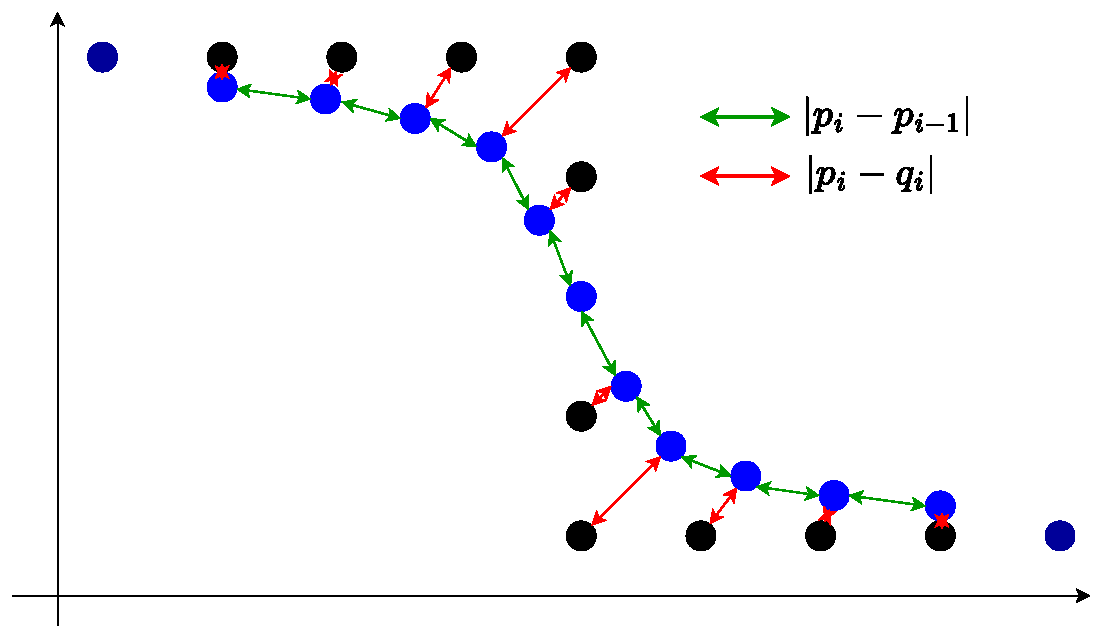
\includegraphics[width=\textwidth]{Figures/PathSmoothing.pdf}
      \end{figure}
    \end{column}
    \begin{column}{0.5\textwidth}
      Considere la función de costo:
      \[J = \alpha\frac{1}{2}\sum_{i=1}^{n-1}\left(p_i - p_{i-1}\right)^2 + \beta\frac{1}{2}\sum_{i=1}^{n-1}(p_i - q_i)^2\]
      \begin{itemize}
      \item $J$ es la suma de distancias entre un punto y otro de la ruta suavizada, y entre la ruta suavizada y la original.
      \item Si la ruta es muy suave, $J$ es grande.
      \item Si la ruta es muy parecida a la original, $J$ también es grande.
      \item Una ruta ni muy suave ni muy parecida a la original, logrará minimizar $J$.
      \end{itemize}
    \end{column}
  \end{columns}
\end{frame}

\begin{frame}\frametitle{Suavizado mediante descenso del gradiente}
  \begin{itemize}
  \item Una forma de encontrar el mínimo es resolviendo $\nabla J(p) = 0$, y luego evaluando la matriz Hessiana para determinar si el punto crítico $p_c$ es un mínimo.
  \item Esto se puede complicar debido al alto número de variables en $p$.
  \item Una forma más sencilla, es mediante el descenso del gradiente.
  \end{itemize}
  \begin{columns}
    \begin{column}{0.7\textwidth}
  \begin{algorithm}[H]
    \footnotesize
  \DontPrintSemicolon
  \KwData {Función $J(p):\mathbb{R}^n\rightarrow \mathbb{R}$ a minimizar}
  \KwResult{Vector $p$ que minimiza la función $J$}
  $p\leftarrow p_{init}$ //Fijar una estimación inicial\;
  \While{$|\nabla J(p)| > tol$}
  {
    $p \leftarrow p - \epsilon \nabla J (p)$ //$p$ se modifica un poco en sentido contrario al gradiente.\;
  }
  Devolver $p$
  \caption{Descenso del gradiente}
\end{algorithm}
\end{column}
\end{columns}
\[\]
El descenso del gradiente devuelve el mínimo local más cercano a la condición inicial $p_0$. Pero la función de costo $J$ tiene solo un mínimo global. El gradiente de la función de costo $J$ se calcula como:
  \[\underbrace{\left[\frac{}{}\alpha(p_0 - p_1)+\beta(p_0 - q_0)\right. }_{\dfrac{\partial J}{\partial p_0}}
,\dots ,
\underbrace{\frac{}{}\alpha(2p_i - p_{i-1} - p_{i+1})+\beta(p_i - q_i)}_{\dfrac{\partial J}{\partial p_i}}
,\dots ,
\underbrace{\left.\alpha(p_{n-1} - p_{n-2})+\beta(p_{n-1}-q_{n-1})\frac{}{}\right]}_{\dfrac{\partial J}{\partial p_{n-1}}}
\]
\end{frame}

\begin{frame}\frametitle{Suavizado mediante descenso del gradiente}
  
  Para no variar los puntos inicial y final de la ruta, la primer y última componentes de $\nabla J$ se dejarán en cero. El algoritmo de descenso del gradiente queda como:
  \[\]
\begin{algorithm}[H]
\DontPrintSemicolon
  \DontPrintSemicolon
  \KwData{Conjunto de puntos $Q = \{q_0\dots q_i \dots q_{n-1}\}$ de la ruta original, parámetros $\alpha$ y $\beta$, ganancia $\epsilon$ y tolerancia $tol$\;}
  \KwResult{Conjunto de puntos $P = \{p_0\dots p_i \dots p_{n-1}\}$ de la ruta suavizada\;}
  $P \leftarrow Q$\;
  $\nabla J_0 \leftarrow 0$\;
  $\nabla J_{n-1} \leftarrow 0$\;   
  \While{ $\Vert\nabla J(p_i)\Vert > tol$}
  {
    \ForEach{$i \in [1,n-1)$}
    {
      $\nabla J_i \leftarrow \alpha (2p_i - p_{i-1} - p_{i+1}) + \beta (p_i - q_i)$\;
    }
    $P \leftarrow P - \epsilon \nabla J$
  }
  regresar $P$
  \caption{Suavizado de rutas mediante descenso del gradiente}
\end{algorithm}
\end{frame}

\begin{frame}[containsverbatim]\frametitle{Ejercicio 05 - Planeación y seguimiento de rutas}
  Realice lo siguiente:
  \begin{enumerate}
     \item Abra el archivo \texttt{catkin\_ws/src/students/scripts/assignment05.py} y agregue el siguiente código en la línea 39:
  \begin{lstlisting}[language=Python,firstnumber=39]
nabla[0], nabla[-1] = 0, 0
while numpy.linalg.norm(nabla) > tol*len(P) and steps < 100000:
    for i in range(1, len(Q)-1):
       nabla[i] =alpha*(2*P[i] - P[i-1] - P[i+1]) + beta*(P[i] - Q[i])
    P = P - epsilon*nabla
    steps += 1
  \end{lstlisting}
  \item Corra la simulación igual en los ejercicios anteriores anteriores. 
  \item Corra los nodos de inflado de mapas, mapa de costo, A* y seguimiento de rutas.
  \item Corra el suavizado de rutas mediante el comando:
    \begin{verbatim}
  rosrun students assignment05.py _alpha:=0.9 _beta:=0.1
\end{verbatim}
  \item En el visualizador, observe la diferencia entre la ruta original calculada con A* (en azul) y la ruta suavizada (en verde). 
  \end{enumerate}
\end{frame}


\begin{frame}[containsverbatim]\frametitle{Ejercicio 05 - Planeación y seguimiento de rutas}
  \begin{enumerate}
    \setcounter{enumi}{5}
    \item Detenga el suavizado de rutas y vuelva a ejecutar con diferentes valores de $\alpha$ y $\beta$.
  \item Detenga el suavizado de rutas y sintonice las constantes $\alpha$ y $\beta$ del control de posición (ejercicio 04) hasta que el robot siga muy de cerca la ruta calculada (no importa que tenga cambios abruptos de velocidad).
  \item Ejecute el suavizado de rutas y el control de posición con las constantes sintonizadas.
  \item Comente los resultados.
  \end{enumerate}
\end{frame}


\begin{frame}\frametitle{Evasión de obstáculos}
  \begin{itemize}
  \item Hasta el momento se tiene una manera de representar el ambiente, planear una ruta y seguirla
  \item ¿Qué pasa si en el ambiente hay un obstáculo que no estaba en el mapa?
  \item Se requiere de una técnica reactiva para evadir obstáculos
  \item Una posible solución es el uso de campos potenciales artificiales
  \end{itemize}
\end{frame}

\begin{frame}\frametitle{Campos potenciales artificiales}
  El objetivo de esta técnica es diseñar una función $U(q):\mathbb{R}^n\rightarrow \mathbb{R}$ que represente energía potencial.
  \begin{itemize}
  \item El gradiente $\nabla U(q) = \left[\frac{\partial U}{\partial q_1},\dots,\frac{\partial U}{\partial q_n}\right]$ es una fuerza.
  \item Se debe diseñar de modo que tenga un mínimo global en el punto meta y máximos locales en cada obstáculo.
  \item Si el robot se mueve siempre en sentido contrario al gradiente $\nabla U$ llegará al punto meta siguiendo una ruta alejada de los obstáculos.
  \item Ha varias formas de diseñar la función $U(q)$, algunas son:
    \begin{itemize}
    \item Algoritmo \textit{wavefront}, requiere una discretización del espacio (requiere mapa previo), pero no presenta mínimos locales.
    \item Campos atractivos y repulsivos, no requieren mapa previo, pero pueden presentar mínimos locales. 
    \end{itemize}
  \end{itemize}
\end{frame}

\begin{frame}\frametitle{Potenciales atractivos y repulsivos}
  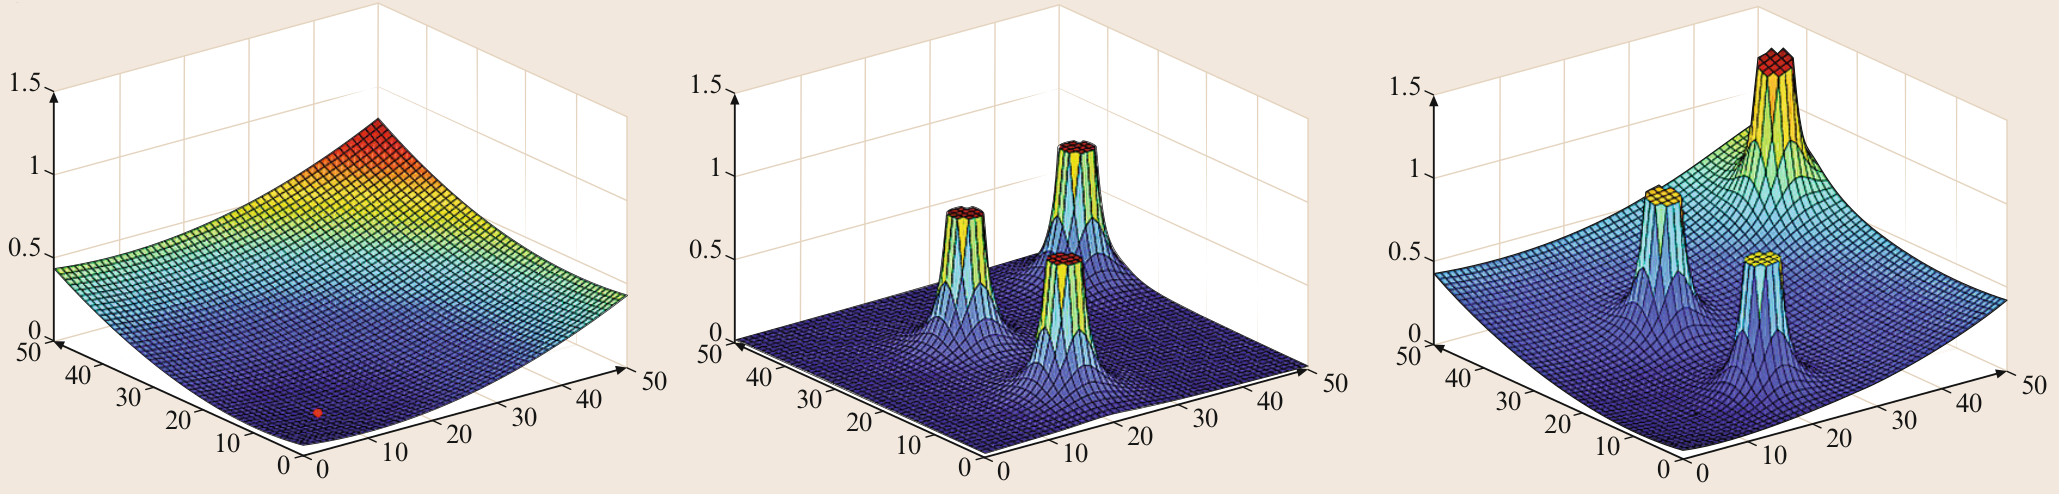
\includegraphics[width=\textwidth]{Figures/PotFieldsExample.png}
  \begin{itemize}
  \item \textbf{Campos repulsivos:} Por cada obstáculo se diseña una función $U_{rej_i}(q)$ con un máximo local en la posición $q_{o_i}$ del obstáculo.
  \item \textbf{Campo atractivo:} Se diseña una función $U_{att}(q)$ con un mínimo global en el punto meta $q_g$.
  \item La función potencial total $U(q)$ se calcula como
    \[ U(q) = U_{att}(q) + \frac{1}{N}\sum_{i=1}^N U_{rej_i}(q)\]
  \end{itemize}
\end{frame}

\begin{frame}\frametitle{Fuerzas atractiva y repulsivas}
  Puesto que el gradiente es un operador lineal, se pueden diseñar directamente las fuerzas atractiva $F_{att}(q) = \nabla U_{att}(q)$ y repulsivas $F_{rej_i}(q) = \nabla U_{rej_i}(q)$, de modo que la fuerza total será:
  \[ \nabla U(q) = F(q) = F_{att}(q) + \frac{1}{N}\sum_{i=1}^N F_{rej_i}(q)\]
  Una propuesta de estas fuerzas es:
  \begin{eqnarray*}
    \label{eq:attractive}
    F_{att} &=& \zeta \dfrac{\left(q - q_g\right) }{\Vert q - q_g \Vert},\qquad \zeta > 0\label{eq:PotFieldsAttraction}\\
    F_{rej} &=& \begin{cases}
                  \eta\left(\sqrt{\dfrac{1}{d} - \dfrac{1}{d_0}}\right)\dfrac{q_{o_i} - q}{d}
                  & \quad\textrm{si}\quad d < d_0\\
                  0 & \quad\textrm{en otro caso}
                \end{cases}
  \end{eqnarray*}
  donde
  \begin{itemize}
  \item $q=(x,y)$ es la posición del robot
  \item $q_g=(x_g, y_g)$ es el punto que se desea alcanzar
  \item $q_{o_i} = (x_{o_i}, y_{o_i})$ es la posición del $i$-ésimo obstáculo
  \item $d_0$ es una distancia de influencia. Más allá de $d_0$ los obstáculos no producen efecto alguno
  \item $\zeta$ y $\eta$, junto con $d_0$, son constantes de sintonización
  \end{itemize}
\end{frame}


\begin{frame}\frametitle{Evasión de obstáculos por campos potenciales}
  \begin{itemize}
  \item Aunque las ecuaciones anteriores suponen que se conoce la posición de cada obstáculo $q_{o_i}$, en realidad ésta aparece siempre en la diferencia $q_{o_i} - q$, es decir, solo se requiere su posición relativa al robot.
  \item Los campos potenciales se implementan utilizando el lidar, donde cada lectura se considera un obstáculo. 
  \end{itemize}
  \begin{figure}
    \centering
    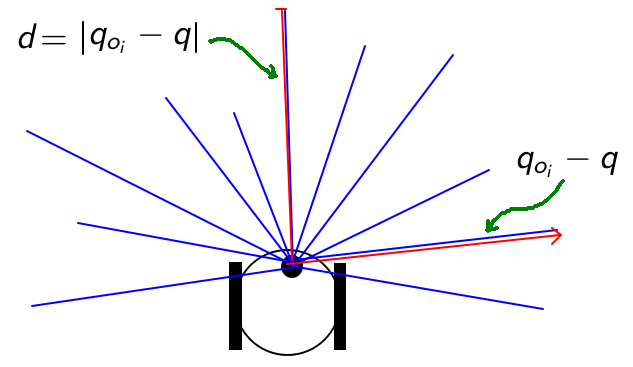
\includegraphics[width=0.4\textwidth]{Figures/PotFieldsLidar.png}
  \end{figure}
  Las lecturas del lídar generalmente son pares distancia-ángulo $(d_i,\theta_i)$ expresados con respecto al robot, por lo que, si se conoce la posición del robot $(x_r,y_r,\theta_r)$, la posición de cada obstáculo se puede calcular como:
  \begin{eqnarray*}
    x_{oi} &=& x_r + d_i\cos(\theta_i + \theta_r)\\
    y_{oi} &=& y_r + d_i\sin(\theta_i + \theta_r)\\
  \end{eqnarray*}
\end{frame}

\begin{frame}\frametitle{Evasión de obstáculos por campos potenciales}
  Finalmente, para que el robot alcance el punto de menor potencial, se puede emplear el descenso del gradiente:
  \[\]
  \begin{algorithm}[H]
  \DontPrintSemicolon
  \KwData{Posición inicial $q_s$, posición meta $q_g$, posiciones $q_{oi}$ de los obstáculos y tolerancia $tol$}
  \KwResult{Secuencia de puntos $\{q_0,q_1, q_2, \dots\}$ para evadir obstáculos y alcanzar el punto meta}
  \;
$q \leftarrow q_s$\;
\While{$\Vert\nabla U(q)\Vert > tol$}
{
  $q \leftarrow q - \epsilon F(q)$\;
  $[v,\omega] \leftarrow $ leyes de control con $q$ como posición deseada\;
}
  \caption{Descenso del gradiente para mover al robot a través de un campo potencial.}
  \label{alg:PotFields}
\end{algorithm}
\end{frame}

\begin{frame}\frametitle{Evasión de obstáculos por campos potenciales}
  Ejemplo de movimiento:
  \begin{figure}
    \centering
    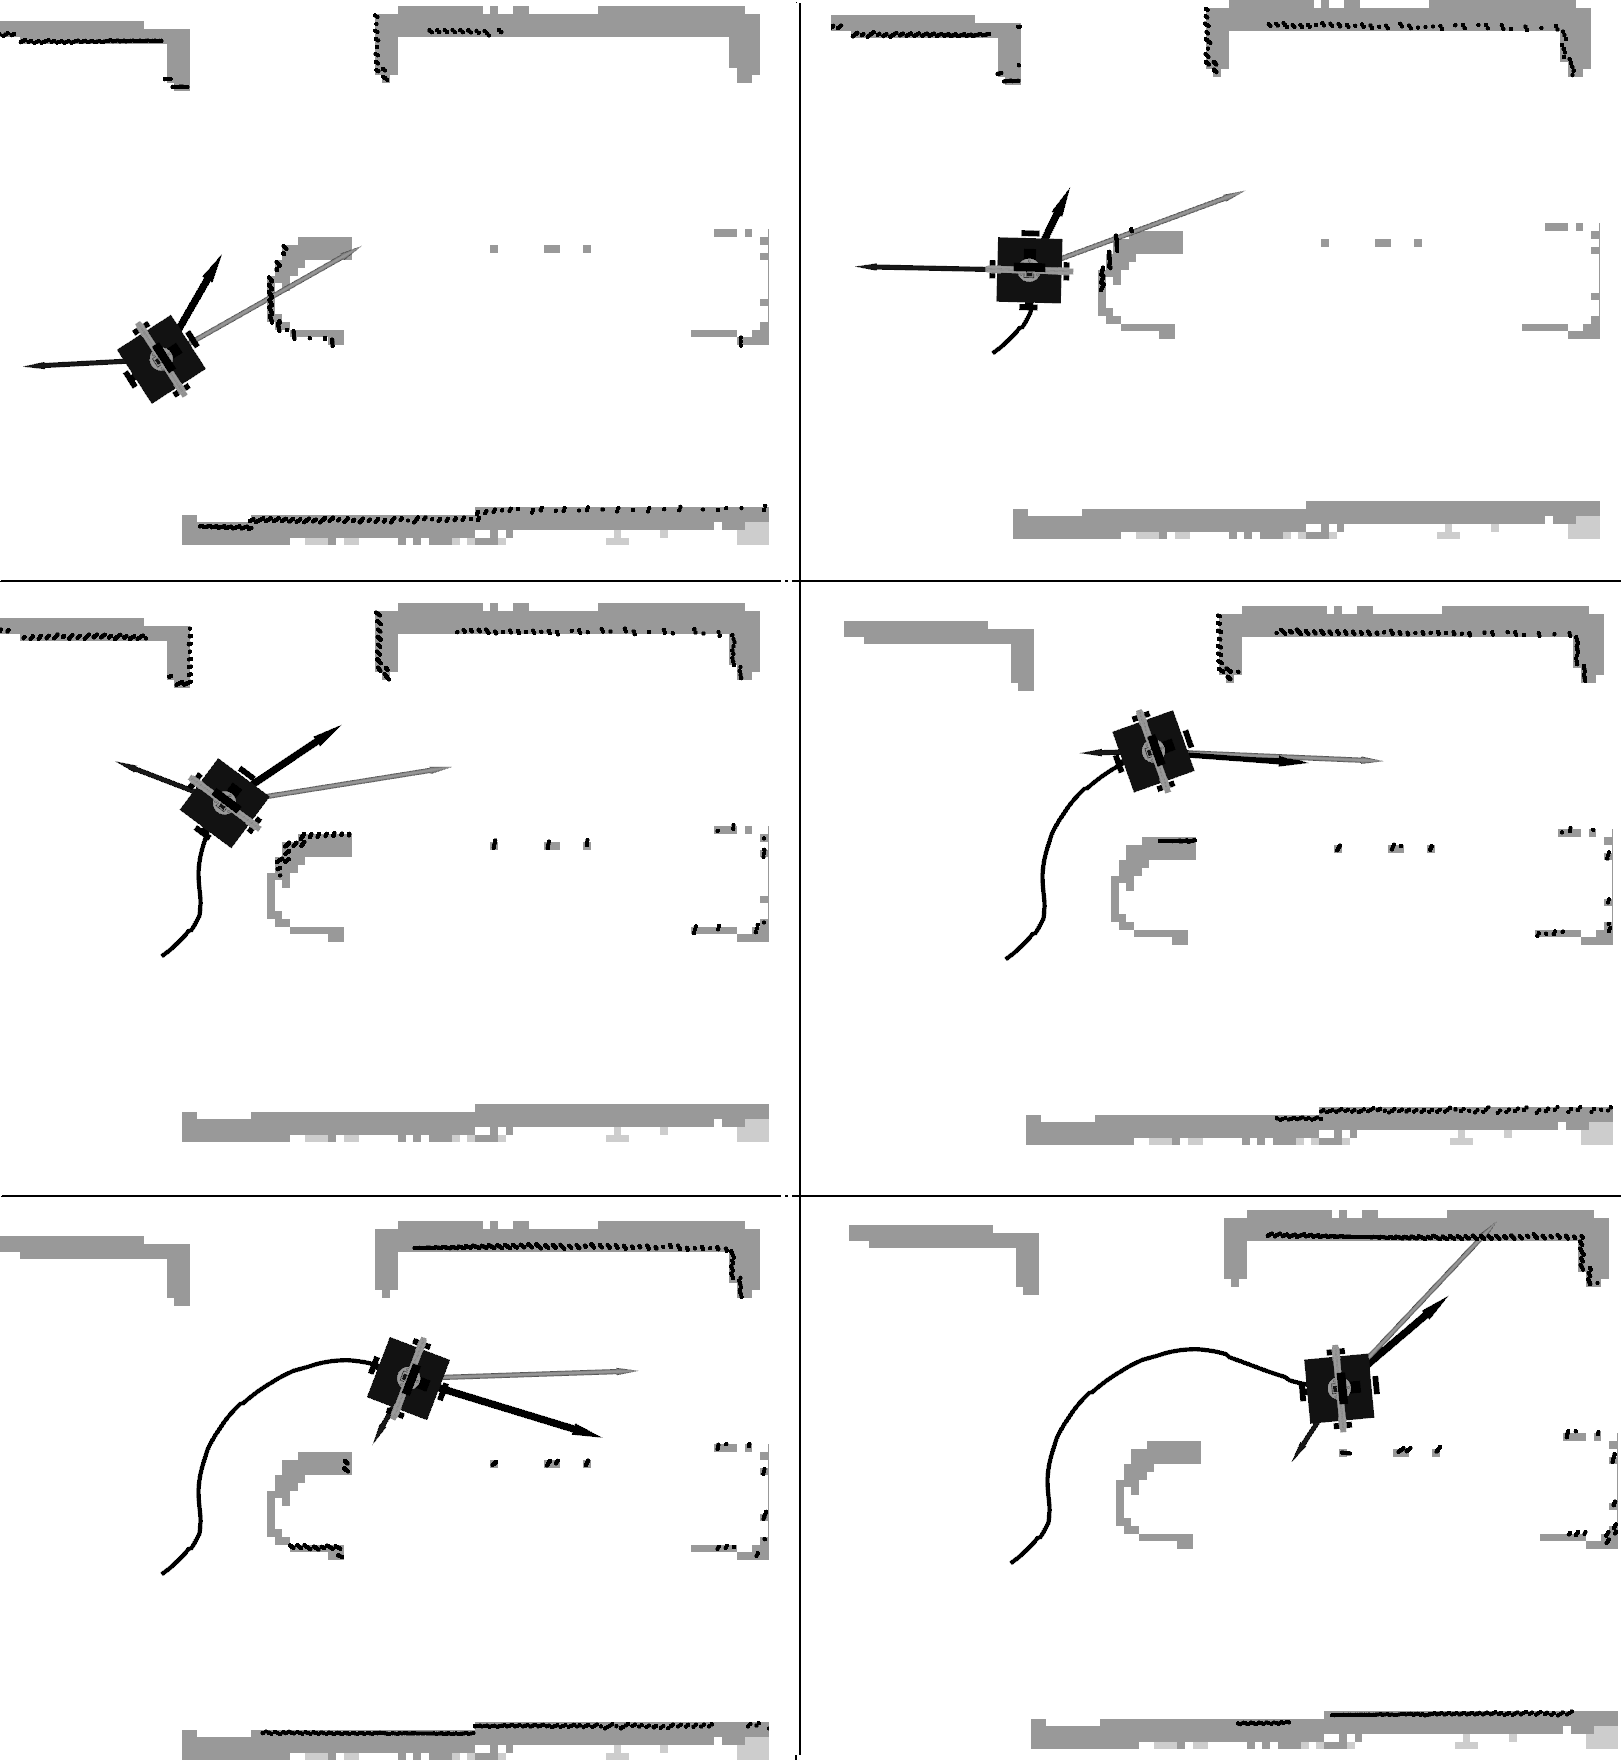
\includegraphics[height=0.85\textheight]{Figures/PotFieldsExecution.png}
  \end{figure}
\end{frame}

\begin{frame}[containsverbatim]\frametitle{Ejercicio 06 - Evasión de obstáculos}
Realice lo siguiente:
  \begin{enumerate}
  \item Abra el archivo \texttt{catkin\_ws/src/students/scripts/assignment06.py} y realice lo siguiente:
    \begin{enumerate}
    \item En la función \texttt{calculate\_control} implemente el control de posición utilizado en la práctica 03
    \item Implemente el cálculo de la fuerza atractiva en la función \texttt{attraction\_force}
    \item En la función \texttt{rejection\_force}, implemente el cálculo de la fuerza repulsiva total
      \[F_{rej} = \frac{1}{N}\sum_{i=1}^N F_{rej_i}(q)\]
      Considere que dada lectura del láser es un obstáculo, como se explicó anteriormente.
    \item En la función \texttt{callback\_pot\_fields\_goal} implemente el descenso del gradiente para mover el robot hacia el punto meta mediante campos potenciales artificiales. Revise los comentarios en el archivo. 
    \end{enumerate}
  \item Ejecute la simulación con el comando
    \begin{verbatim}
   roslaunch surge_et_ambula obstacle_avoidance.launch
\end{verbatim}
  \item Ejecute la evasión por campos potenciales mediante el comando
\begin{verbatim}
   rosrun students assignment06.py
\end{verbatim}
  \item Con la opción \textit{2D Nav Goal} del visualizador \textit{RViz}, selecccione un punto meta en el mapa.
  \item Observe qué sucede.
  \item Pruebe con diferentes constantes de sintonización y observer los cambios en el comportamiento. 
  \end{enumerate}
\end{frame}

\begin{frame}\frametitle{Localización}
  El problema de la localización consiste en determinar la configuración $q$ del robot dada un mapa y un conjunto de lecturas de los sensores.
  \begin{itemize}
  \item La localización se podría lograr simplemente integrando los comandos de velocidad del robot.
  \item Si se conoce perfectamente la configuración inicial y el robot ejecuta perfectamente los comandos de movimiento, entonces la simple integración de la velocidad de los motores sería suficiente.
  \item Esto por supuesto no es posible. Se tiene incertidumbre tanto en la estimación inicial de la posición como en la ejecución de cada movimiento.
  \item Es decir, el robot pierde información sobre su posición en cada movimiento. 
  \end{itemize}
\end{frame}

\begin{frame}\frametitle{Localización}
  Existen principalmente dos tipos:
\[\]
  \begin{columns}
    \begin{column}{0.5\textwidth}
      \textbf{Localización local: }
      \begin{itemize}
      \item Requiere una estimación inicial \textit{cercana} a la posición real del robot, de otro modo, no converge.
      \item Suele ser menos costosa computacionalmente.
      \item Un método común es el Filtro de Kalman Extendido.
      \end{itemize}
    \end{column}
    \begin{column}{0.5\textwidth}
      \textbf{Localización global:}
      \begin{itemize}
      \item La estimación inicial puede ser cualquiera.
      \item Suele ser computacionalmente costosa.
      \item Un método común son los Filtros de Partículas. 
      \end{itemize}
      \[\]
      \[\]
    \end{column}
  \end{columns}
\end{frame}

\begin{frame}\frametitle{Localización probabilística}
  \begin{itemize}
  \item En la localización probabilística, en lugar de llevar una sola hipótesis sobre la posición del robot, se mantiene una \textit{distribución de probabilidad} sobre todo el espacio de hipótesis.
  \item El enfoque probabilístico permite manejar las incertidumbres inherentes al movimiento y al sensado.
  \item El reto es obtener una distribución de densidad de probabilidad (PDF) sobre todas las posibles posiciones del robot.
  \item En general, los métodos probabilísticos de estimación se componen de dos pasos:
    \begin{enumerate}
    \item \textbf{Predicción:} Se modifica la PDF de la posición del robot con base en los comandos y el modelo de movimiento.
    \item \textbf{Actualización:} Se corrige la predicción mezclando la información de PDF predicha con información de los sensores. Se obtiene una PDF de la posición y se repite el proceso. 
    \end{enumerate}
  \end{itemize}
  
\end{frame}

%%%%%%%%%%%%%%%%%%%
%%% 2023-03-23 %%%%
%%%%%%%%%%%%%%%%%%%
\section{Filtro de Kalman Extendido (2023-03-23)}
\begin{frame}\frametitle{El Filtro de Kalman Extendido}
\end{frame}

\begin{frame}\frametitle{Algoritmo de estimación del EKF}
\end{frame}

\begin{frame}\frametitle{Tarea 07 - Filtro de Kalman Extendido}
\end{frame}

%%%%%%%%%%%%%%%%%%%
%%% 2023-03-28 %%%%
%%%%%%%%%%%%%%%%%%%
\section{Filtro de Kalman Extendido (2023-03-28)}
\begin{frame}\frametitle{Modelo cinemático discreto}
\end{frame}

\begin{frame}\frametitle{Modelo de observación}
\end{frame}

\begin{frame}\frametitle{Extracción de marcas}
\end{frame}

\begin{frame}\frametitle{Obtención de las matrices $Q$ y $R$}
\end{frame}

% \begin{frame}\frametitle{Práctica 06 - Filtro de Kalman Extendido}
% \end{frame}


%%%%%%%%%%%%%%%%%%%
%%% 2023-03-30 %%%%
%%%%%%%%%%%%%%%%%%%
\section{Filtro de Partículoas (2023-03-30)}
  
\begin{frame}\frametitle{Filtros de Partículas}
  \begin{figure}
    \centering
    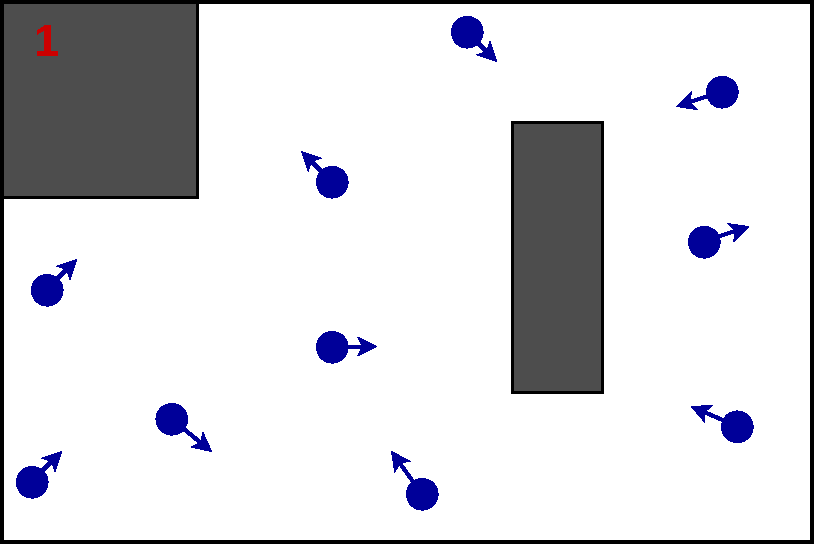
\includegraphics[width=0.6\textwidth]{Figures/ParticleFilter1.pdf}
  \end{figure}
\end{frame}

\begin{frame}\frametitle{Tarea 08 - Conceptos de filtros de partículas}
  \begin{itemize}
  \item Ejercicio de remuestreo con reemplazo
  \item Transformación de posición par desplazamiento de las partículas
  \end{itemize}
\end{frame}

%%%%%%%%%%%%%%%%%%%
%%% 2023-04-11 %%%%
%%%%%%%%%%%%%%%%%%%
\section{Filtros de partículas (2023-04-11)}

\begin{frame}\frametitle{Simulación del sensor}
\end{frame}

\begin{frame}\frametitle{Comparación de simulación con real}
\end{frame}

\begin{frame}\frametitle{Remuestreo con reemplazo}
\end{frame}

\begin{frame}\frametitle{Desplazamiento de partículas}
\end{frame}

\begin{frame}\frametitle{Tarea 09 - Ejercicios de filtros de partículas}
  \begin{itemize}
  \item Ejercicio de remuestreo con reemplazo
  \item Transformación de posición par desplazamiento de las partículas
  \end{itemize}
\end{frame}

%%%%%%%%%%%%%%%%%%%
%%% 2023-04-13 %%%%
%%%%%%%%%%%%%%%%%%%
\section{Filtros de partículas (2023-04-13)}

\begin{frame}\frametitle{Repaso de C++}
\end{frame}

\begin{frame}\frametitle{La biblioteca \textit{random\_numbers}}
\end{frame}

\begin{frame}[containsverbatim]\frametitle{Práctica 05 - Localización por filtros de partículas}
Realice lo siguiente:
  \begin{enumerate}
  \item Abra el archivo \texttt{catkin\_ws/src/students/src/practice05.cpp} y realice lo siguiente:
    \begin{enumerate}
    \item En la función \texttt{get\_initial\_distribution} genere $N$ partículas con pose $(x,y,\theta)$ aleatoria con distribución uniforme. 
    \item Complete la función \texttt{simulate\_particle\_scans} para generar lecturas del láser simuladas dado un mapa y la posición de las partículas. 
    \item En la función \texttt{calculate\_particle\_similarities}, calcule la similitud vista en clase para cada partícula y normalice los valores para sumen 1.
    \item Complete la función \texttt{random\_choice} para devolver un índice aleatorio $i$ dada una distribución de probabilidad cualquiera determinada por un arreglo de probabilidades $p$.
    \item En la función \texttt{resample\_particles} implemente el remuestreo con reemplazo visto en clase, dado un conjunto de partículas y una distribución de probabilidad.
    \item En la función \texttt{move\_particles} implemente el movimiento de partículas dado un desplazamiento.
    \item Complete la función \texttt{main} de acuerdo con las instrucciones dadas en los comentarios del código. 
    \end{enumerate}
  \item Compile el código con el comando \texttt{catkin\_make} (el directorio de trabajo debe ser \texttt{catkin\_ws})
  \item Ejecute la simulación con el comando \texttt{roslaunch bring\_up localization.launch}
  \item Corra la práctica con el comando \texttt{rosrun students practice05}
  \item Mueva el robot con la GUI y observe lo que sucede en el visualizador. 
  \item El código debe recompilarse con cada cambio. 
  \end{enumerate}
\end{frame}

\begin{frame}[containsverbatim]\frametitle{Práctica 05 - Localización por filtros de partículas}
 \textbf{Entregables:}
  \begin{itemize}
  \item Código modificado en la rama correspondiente del repositorio en línea.
  \item Documento escrito con los puntos indicados al inicio del semestre
  \end{itemize}
  \textbf{Deadline: } 2023-05-09 al inicio de la clase. 
\end{frame}



% %%%%%%%%%%%%%%%%%%%
% %%% 2023-04-18 %%%%
% %%%%%%%%%%%%%%%%%%%
% \section{Creación de mapas (2023-04-18)}

% \begin{frame}\frametitle{Agrupamiento}
% \end{frame}

% \begin{frame}\frametitle{K-medias}
% \end{frame}

% \begin{frame}\frametitle{Cuantización vectorial}
% \end{frame}

% \begin{frame}\frametitle{Tarea 10 - Investigación agrupamiento}
% \end{frame}

% %%%%%%%%%%%%%%%%%%%
% %%% 2023-04-20 %%%%
% %%%%%%%%%%%%%%%%%%%
% \section{Localización y mapeo simultáneos (2023-04-20)}

% \begin{frame}\frametitle{Localización y mapeo simultáneos}
% \end{frame}

% \begin{frame}\frametitle{Práctica 8 - SLAM}
% \end{frame}


\section{Visión artificial}

\begin{frame}\frametitle{¿Qué es la visión computacional?}
  \begin{itemize}
  \item \textbf{Visión Humana: } Se puede concebir como una tarea de procesamiento de información, que obtiene significado a partir de los estímulos percibidos por los ojos.
  \item \textbf{Visión Computacional: } Desarrollo de programas de computadora que puedan \textit{interpretar} imágenes. Es decir, realizar la visión humana por medios computacionales. 
  \end{itemize}
  \begin{figure}
    \centering
    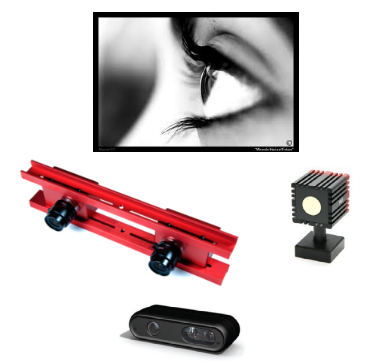
\includegraphics[width=0.5\textwidth]{Figures/ComputerVision.png}
  \end{figure}
\end{frame}

\begin{frame}\frametitle{Teoría de Marr}
“Visión es un proceso que produce, a partir de imágenes del mundo externo, una descripción que es útil para el observador y que está libre de información irrelevante.” (Marr, 1976).\\
El fenómeno de la visión lo podemos considerar como el producto de un sistema de procesamiento de información.\\

Marr propone los siguientes tres niveles de construcción de un sistema de procesamiento de información:\\
\begin{enumerate}
\item Teoría Computacional (¿Cuál es el problema por resolver?)
\item Representación y algoritmos (Estrategía usada para resolverlo)
\item Implementación (Realización física, software y hardware)
\end{enumerate}
Es decir, la visión computacional sería un proceso parecido a la visión humana, similar en los niveles computacionales y de algoritmos, pero implementado de forma diferente: en hardware de procesamiento con sensores de visión. 
\end{frame}

\begin{frame}\frametitle{Visión Computacional}
  Por lo tanto, la tarea de la Visión por computadora es la construcción de descriptores de la escena con base en características relevantes contenidas en una imagen:
  \begin{columns}
    \begin{column}{0.5\textwidth}
\begin{figure}
    \centering
    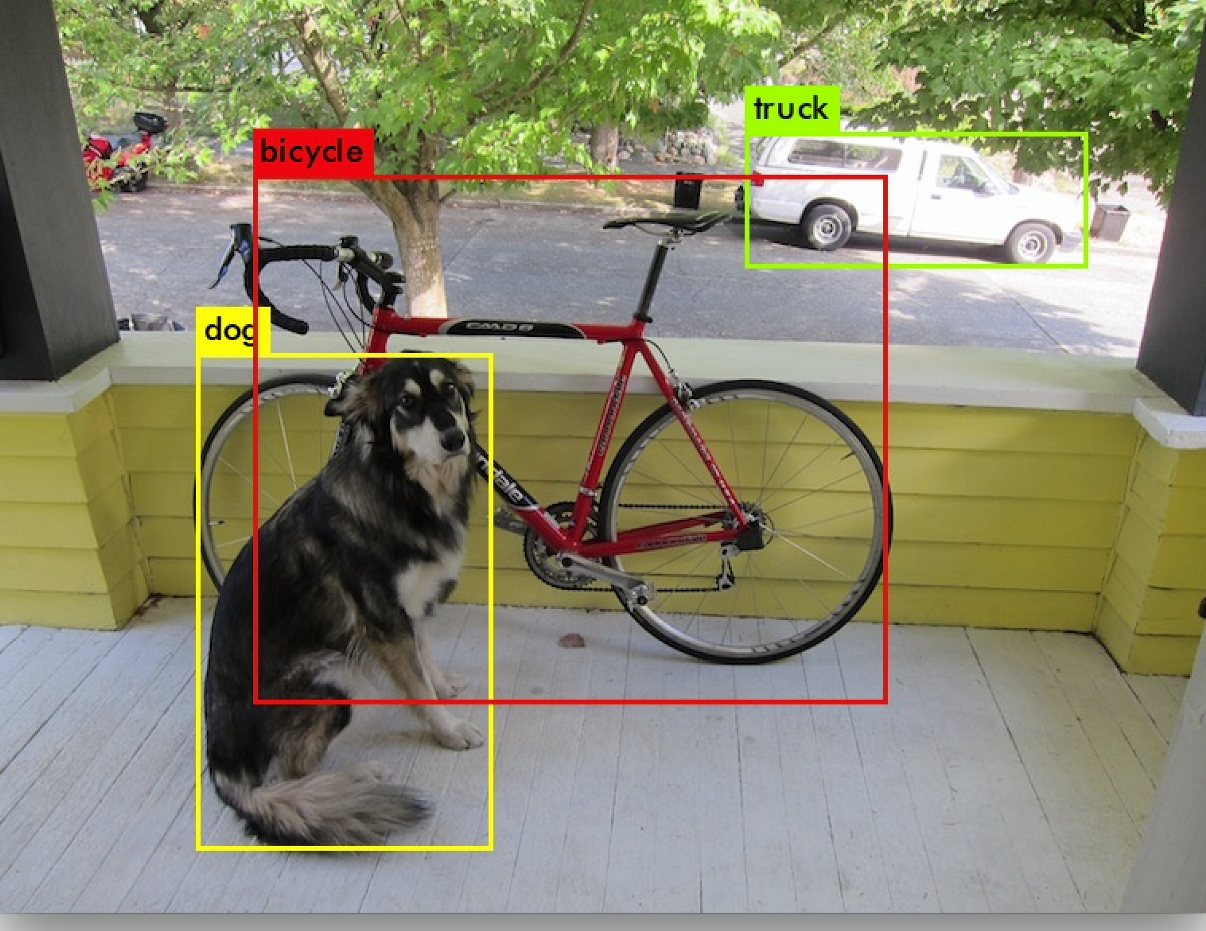
\includegraphics[width=0.8\textwidth]{Figures/YoloExample.png}
\end{figure}
    \end{column}
    \begin{column}{0.5\textwidth}
\begin{itemize}
\item Objetos
\item Formas de Superficies
\item Colores
\item Texturas
\item Movimientos
\item Iluminación
\item Reflejos
\end{itemize}
    \end{column}
    \end{columns}
\end{frame}

\begin{frame}\frametitle{Vision Computacional vs Proc de Imágenes}
\begin{enumerate}
\item Procesamiento de imagenes: Es cualquier forma de procesamiento de señales donde la entrada es una imagen, la salida puede ser otra imagen o un conjunto de características o parámetros relacionados con la misma.
\item Visión Computacional: Estudio y aplicación de métodos que permiten a las computadoras “entender” el contenido de una imagen.
\item Visión Máquina: Es la aplicación de la visión por computadora en la industria y procesos de manufactura.
\end{enumerate}

\end{frame}

\begin{frame}\frametitle{Aplicaciones}
  Tareas que se pueden hacer con visión computacional (con aplicaciones a la robótica):
  \begin{itemize}
  \item OCR (Optical Character Recognition)
  \item Detección e identificación de rostros
  \item Reconocimiento de objetos
  \item Percepción para vehículos sin conductor
  \item Reconocimiento de gestos
  \end{itemize}
  Otras aplicaciones:
  \begin{itemize}
  \item Vigilancia
  \item Imagenología médica
  \item Consultas a bases de datos de imágenes.
  \item Percepción remota
  \end{itemize}
\end{frame}


\begin{frame}\frametitle{Esquema de Visión}
  \begin{figure}
    \centering
    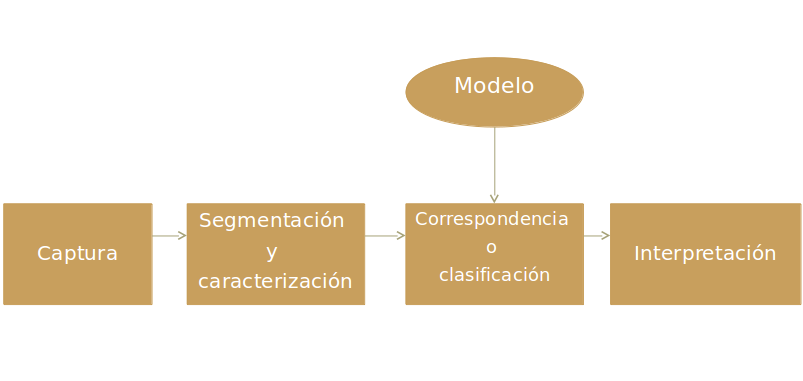
\includegraphics[width=1.0\textwidth]{Figures/VisionGeneralProcess.png}
  \end{figure}
\end{frame}


\begin{frame}\frametitle{Dificultades}

  El entorno real tiene una gran cantidad de variaciones en las imágenes de entrada.
  \begin{columns}
    \begin{column}{0.5\textwidth}
\begin{figure} %this figure will be at the right
    \centering
    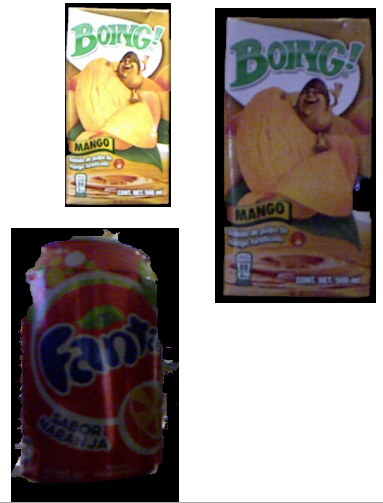
\includegraphics[width=0.5\textwidth]{Figures/ComputerVisionProblems.png}
\end{figure}
    \end{column}
    \begin{column}{0.5\textwidth}
\begin{enumerate}
\item Iluminación
\item Orientación
\item Oclusión
\item Escala
\item Ruido
\item Desenfoque
\end{enumerate}
    \end{column}
  \end{columns}
\end{frame}

\begin{frame}\frametitle{Hardware y Software}
La computación con imágenes tiene mas de 30 años, sin embargo, en los últimos años, se ha incrementado considerablemente su desarrollo debido a:
\begin{enumerate}
\item Decremento en los precios 
\item Memoria con gran capacidad
\item Procesadores de propósito general de alta velocidad.
\item Existen scanners o camaras digitales que pueden ser utilizados para procesar imágenes propias.
\item Existen bibliotecas de software que contienen subrutinas de procesamiento de imágenes (opencv).
\end{enumerate}
\end{frame}

\begin{frame}\frametitle{OpenCV}
  \begin{columns}
    \begin{column}{0.5\textwidth}
      \begin{figure}
        \centering
        
\includegraphics[width=0.6\textwidth]{Figures/OpenCVLogo.png}
      \end{figure}
    \end{column}
    \begin{column}{0.5\textwidth}
      OpenCV es una biblioteca libre de visión artificial, originalmente desarrollada por Intel.
      
      Programación en código  Python, C y C++
      
      Existen versiones para GNU/Linux, Mac OS X y Windows
    \end{column}
    \end{columns}
    \end{frame}

\begin{frame}\frametitle{OpenCV}
\begin{figure}[h!]
        \centering
        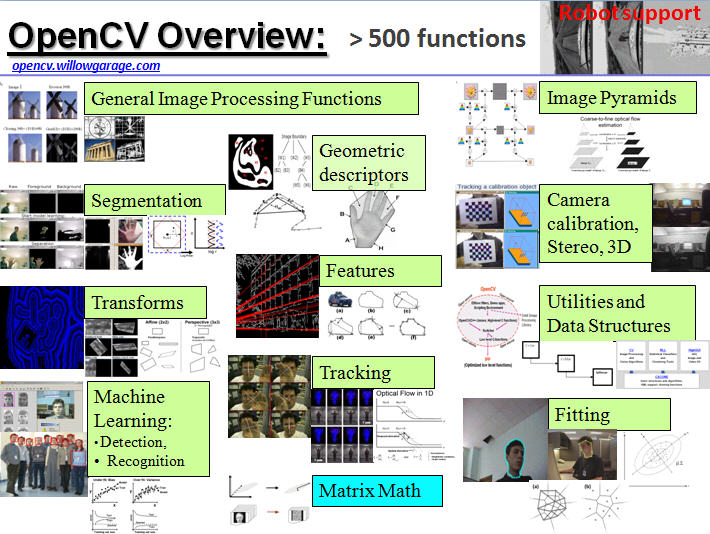
\includegraphics[width=0.75\textwidth]{Figures/OpenCVOverview.png}
\end{figure}
\end{frame}


\begin{frame}\frametitle{Imágenes como funciones}
  \begin{itemize}
  \item Una imagen (en escala de grises) es una función $I(x,y)$ donde $x,y$ son variables discretas en coordenadas de imagen y la función $I$ es intensidad luminosa.
    \item Las imágenes también pueden considerarse como arreglos bidimensionales de números entre un mínimo y un máximo (usualmente 0-255).
    \item Las imágenes de color son funciones vectoriales $f:\mathbb{R}^2\rightarrow \mathbb{R}^3$ donde cada componente de la función se llama canal.
%  \[I(x,y) = \left[\begin{tabular}{c}$r(x,y)$\\$g(x,y)$\\$b(x,y)$\end{tabular}\right]\]
  \end{itemize}
  \begin{figure}
    \centering
    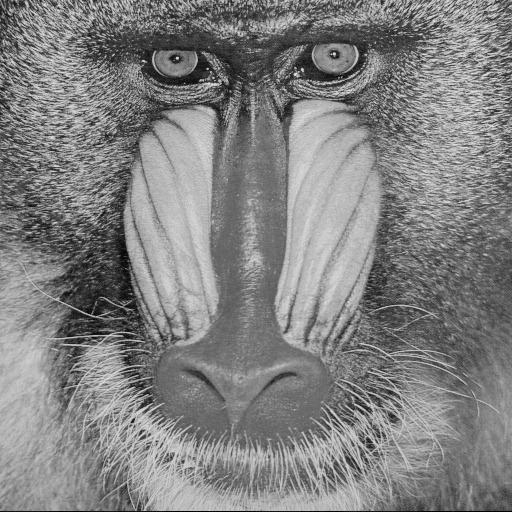
\includegraphics[width=0.3\textwidth]{Figures/baboon_grayscale.jpg}
    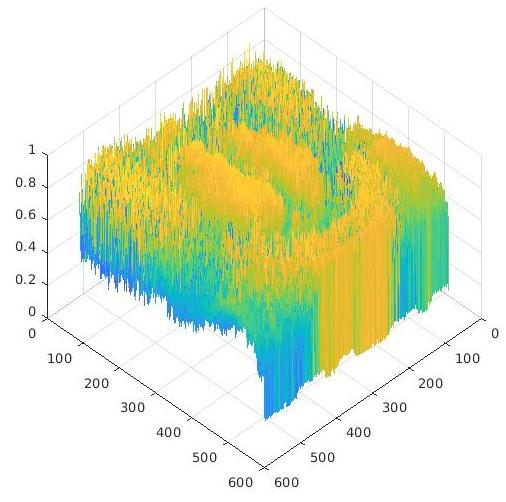
\includegraphics[width=0.35\textwidth]{Figures/BaboonPlot.jpg}
  \end{figure}
\end{frame}

\begin{frame}\frametitle{Las imágenes como funciones}
    Aunque formalmente una imagen es un mapeo $f:\mathbb{R}^2\rightarrow \mathbb{R}$, en la práctica, tanto $x,y$ como $I$ son varialbes discretas con valores entre un mínimo y un máximo.
\begin{figure}
  \centering
  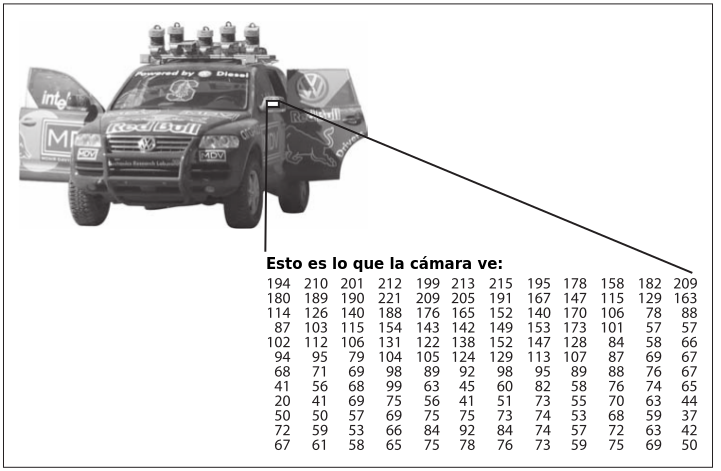
\includegraphics[width=0.45\textwidth]{Figures/ImageRepresentation.png}
\end{figure}
\end{frame}


\begin{frame}\frametitle{Operaciones básicas}
  \begin{itemize}
  \item Desfase
  \item Escalamiento
  \item Inversión en $x,y$
  \item Suma y Resta 
  \item Multiplicación
  \end{itemize}
\end{frame}

\begin{frame}\frametitle{Tipos de ruido}
  El ruido es una señal aleatoria $\eta(x,y)$, es decir, no sabemos cuánto vale para un punto determinado $(x,y)$ pero sí podemos caracterizarla.
  \[I_n(x,y) = I(x,y) + \eta(x,y)\]
  Existen varios tipos de ruido:
  \begin{itemize}
  \item Sal y pimienta: aleatoriamente aparecen puntos ya sea blancos o negros
  \item Ruido de impulso: aleatoriamente aparecen puntos blancos
  \item Ruido gausiano: $\eta(x,y)$ se distribuye normalmente
  \end{itemize}
\end{frame}

% \begin{frame}\frametitle{Tarea 11 - Herramientas de visión artificial}
% \end{frame}

\begin{frame}\frametitle{Espacios de color}
  Un espacio de color o modelo de color es una representación del color mediante un conjunto numérico de valores, generalmente tres valores. Existen varios espacios de color:
  \begin{columns}
    \begin{column}{0.5\textwidth}
      \begin{itemize}
      \item Aditivos:
        \begin{itemize}
        \item RGB
        \item HSV
        \item YCrCb
        \end{itemize}
      \item Sustractivos
        \begin{itemize}
        \item MCYK
        \end{itemize}
      \end{itemize}
    \end{column}
    \begin{column}{0.5\textwidth}
      \begin{itemize}
      \item Lineales:
        \begin{itemize}
        \item RGB
        \item CIE XYZ
        \end{itemize}
      \item No lineales
        \begin{itemize}
        \item HSV
        \item HSI 
        \end{itemize}
      \end{itemize}
    \end{column}
  \end{columns}
\end{frame}

\begin{frame}\frametitle{El espacio RGB}
  En este espacio cada color se forma mediante la suma de tres colores primarios: rojo, verde y azul. 
  \begin{figure}
    \centering
    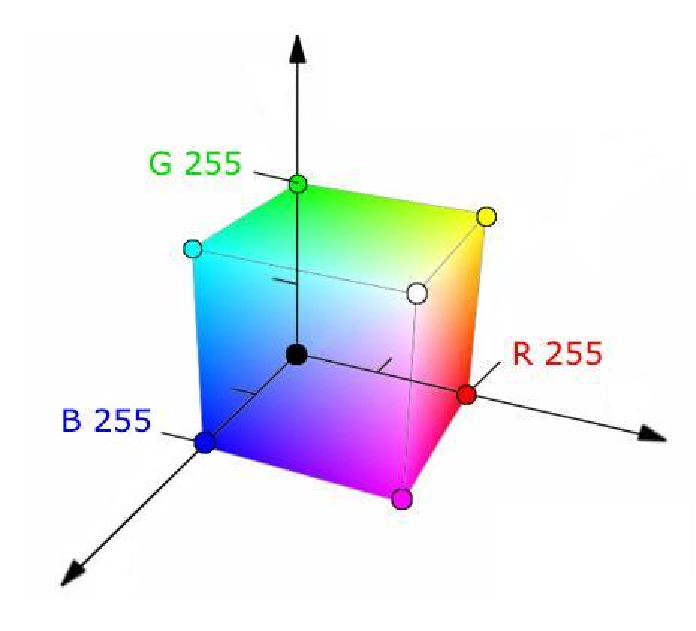
\includegraphics[width=0.33\textwidth]{Figures/RGB_model.pdf}
    \includegraphics[width=0.5\textwidth]{Figures/rgb_pixels.png}
  \end{figure}
  En memoria, las imágenes RGB se suelen representar con arreglos de $H\times W \times 3$ donde $H$ y $W$ son el alto y ancho de la imagen respectivamente. 
\end{frame}

\begin{frame}\frametitle{El espacio HSV}
  Es un espacio de color diseñado para representar el color de una forma más similar a como lo percibe el ojo humano. El color se representa con tres valores:
  \begin{itemize}
  \item \textbf{Hue:} (Matiz) Es el atributo del color que hace que un estímulo se perciba como similar a alguno de los colores que el ojo puede percibir: rojo, amarillo, verde, azul, violeta, o una combinación de ellos.
  \item \textbf{Saturaion: } (Saturación) Es el atributo que indica qué tan colorido es un estímulo con respecto a su propio brillo.
  \item \textbf{Value: } (Valor) Atributo que indica qué tanta luz emite un estímulo. 
  \end{itemize}
  \begin{columns}
    \begin{column}{0.35\textwidth}
      \begin{figure}
        \centering
        \includegraphics[width=\textwidth]{Figures/hsv_space.pdf}
      \end{figure}
    \end{column}
    \begin{column}{0.65\textwidth}
      Para obtenerlo a partir de RGB:
      \[M = \max(R,G,B)\qquad m=\min(R,G,B)\qquad C=M - m\]
      \[H = \begin{cases}\begin{tabular}{lcl}Indeterminado & si & C=0 \\ $\frac{G-B}{C}\times 60$ & si & M = R \\ $\frac{B - R}{C}\times 60$ & si & M = G \\ $\frac{R - G}{C}\times 60$ & si & M = B\end{tabular}\end{cases}\qquad V = M\]
      \[S = \begin{cases}0\qquad \textrm{si}\; V=0\\ \frac{C}{V}\qquad \textrm{en otro caso}\end{cases}\]
    \end{column}
  \end{columns}
\end{frame}

\begin{frame}\frametitle{Nubes de puntos}
  Las nubes de puntos son conjuntos de vectores que representan puntos en el espacio. Estos vectores generalmente tienen información de posición $(x,y,z)$. También pueden contener información de color $(x,y,z,r,g,b)$.
  \begin{figure}
      \centering
      \includegraphics[width=0.5\textwidth]{Figures/CloudExample.png}
  \end{figure}
  Son útiles para determinar la posición en el espacio de los objetos reconocidos. 
\end{frame}

\begin{frame}\frametitle{Segmentación por color}
  La segmentación de una imagen se refiere a obtener regiones significativas con ciertas características. En este caso, la característica es que estén en un cierto intervalo de color. Los pasos generales para esto son:
  \begin{enumerate}
  \item Transformación de la imagen del espacio BGR al HSV (función \texttt{cvtColor})
  \item Obtención de aquellos pixeles que están en un rango de color (función \texttt{inRange})
  \item Eliminación de \textit{outliers}, generalmente con operadores morfológicos (funciones \texttt{erode} y \texttt{dilate})
  \item Obtención del centroide de la región (funciones \texttt{findNonZero} y \texttt{mean})
  \item Si se dispone de una nube de puntos, se puede obtener la posición $(x,y,z)$ del centroide de la región segementada. 
  \end{enumerate}
\end{frame}

\begin{frame}\frametitle{Ejercicio 08 - Segmentación por color}
  \begin{enumerate}
  \item En el archivo \texttt{catkin\_ws/src/students/scripts/assignment08.py}, en la función \texttt{segment\_by\_color}, realice lo siguiente:
    \begin{enumerate}
    \item Defina dos límites superiores y dos límites inferiores, en el espacio de color HSV, para segmentar las latas que se encuentran sobre el escritorio simulado.
    \item Transforme la imagen del espacio BGR al espacio HSV mediante la función \texttt{cvtColor} de OpenCV.
    \item Determine los pixeles de la imagen que pertenecen al rango de color elegido mediante la fucion \texttt{inRange} de OpenCV.
    \item Encuentre los índices de los pixeles que pertenecen al rango de color con la función \texttt{findNonZero} de OpenCV.
    \item Utilizando los índices anteriores y la nube de puntos, determine el centroide del objeto con el color seleccionado. 
    \end{enumerate}
  \item Ejecute la simulación con el comando \texttt{roslaunch bring\_up vision\_examples.launch }
  \item Ejecute la práctica con el comando \texttt{rosrun students assignment08.py}
  \item En la pestaña \textit{Simple Tasks} de la GUI, en el campo \textit{Find Object} teclee \texttt{pringles} o \texttt{drink}
  \item En el visualizador debe dibujarse una esfera morada sobre el centro del objeto seleccionado. 
  \end{enumerate}
\end{frame}

\begin{frame}\frametitle{SLID}
  Un sistema $S$ es un mapeo del conjunto de señales al conjunto de señales, es decir, es algo donde entra una señal $I(x,y)$ y sale otra señal $O(x,y)$:
  \[O(x,y) = S[I(x,y)]\]
  Los sistemas lineales invariantes ante el desfase son sistemas en los que se cumplen las siguientes propiedades:
  \begin{itemize}
  \item \textbf{Aditividad y homogeneidad:}
    \[S[\alpha I_1(x,y) + \beta I_2(x,y)] = \alpha S[I_1(x,y)] + \beta S[I_2(x,y)]\]
  \item \textbf{Invarianza ante el desfase:}
    \[\textrm{Si} \qquad S[I(x,y)] = O(x,y) \qquad\textrm{entonces:}\]
    \[S[I(x-i, y-j)] = O(x-i, y-j) \qquad \forall i,j \in \mathbb{Z}\]
  \end{itemize}
  Los SLID se pueden caracterizar de varias formas:
  \begin{itemize}
  \item Ecuaciones en diferencias
  \item Funciones de transferencia
  \item Respuesta al impulso
  \end{itemize}
\end{frame}

\begin{frame}\frametitle{Convolución}
  Si se conoce la respuesta al impulso $H(x,y)$ de un sistema SLID, se puede obtener la salida $O(x,y)$ ante cualquier entrada $I(x,y)$, mediante la convolución, definida como:
  \[O(x,y) = I(x,y)*H(x,y) = \sum_{i=-\infty}^\infty \sum_{j=-\infty}^\infty I(i,j)H(x-i, y-j)\]
  Ejemplos:
  \[\left[\begin{tabular}{cccc}
      3 & 1 & 4 & 1\\
      5 & 9 & 2 & 6\\
      5 & 3 & 5 & 8\\
      9 & 7 & 9 &3
    \end{tabular}\right]* [1\quad -1] =
  \left[\begin{tabular}{ccccc}
      3 & -2 & 3 & -3 & -1\\
      5 & 4 & -7 & 4 & -6\\
      5 & -2 & 2 & 3 & -8\\
      9 & -2 & 2 & -6 & -3
    \end{tabular}\right]\]

  \[\left[\begin{tabular}{cccc}
      3 & 1 & 4 & 1\\
      5 & 9 & 2 & 6\\
      5 & 3 & 5 & 8\\
      9 & 7 & 9 &3
    \end{tabular}\right]* \left[\begin{tabular}{c}1 \\ -1\end{tabular}\right] =
  \left[\begin{tabular}{cccc}
      3 & 1 & 4 & 1\\
      2 & 8 & -2 & 5\\
      0 & -6 & 3 & 2\\
      4 & 4 & 4 & -5\\
      -9 & -7 & -9 & -3
    \end{tabular}\right]\]
\end{frame}

\begin{frame}\frametitle{Manejo de bordes}
  En el ejemplo anterior, supusimos que fuera de la matriz, todos los elementos son cero. Sin embargo existen otras formas de manejar los borde:
  \begin{itemize}
  \item Recortar: suponer que fuera de la matriz los valores son cero. En el caso de una imagen, suponemos pixeles negros fuera de la imagen.
  \item Wrap around: suponer que la imagen es periódica.
  \item Borde repetido: suponer que los valores de los bordes se mantienen iguales fuera de la imagen.
  \item Reflexión: fuera de los bordes se tiene una imagen en espejo.
  \end{itemize}
\end{frame}

\begin{frame}\frametitle{Propiedades de la convolución}
  \begin{itemize}
  \item Es conmutativa: $H*I = I*H$
  \item Es asociativa: $H*I_1*I_2$ = $H*(I_1*I_2)$ = $(H*I_1)*I_2$
  \item Es distributiva: $H*(I_1 + I_2) = H*I_1 + H*I_2$
  \item Es lineal: $H*(\alpha I_1 + \beta I_2) = \alpha H*I_1 + \beta H*I_2$
  \end{itemize}
  En el caso de secuencias finitas bidimensionales:
  \begin{itemize}
  \item Si $I\in\mathbb{R}^{r_1\times c_1}$ y $H\in\mathbb{R}^{r_2\times c_2}$, entonces $(I*H) \in \mathbb{R}^{(r_1+r_2-1)\times (c_1 + c_2 - 1)}$
  \item Si $I\in\mathbb{R}^{r_1\times c_1}$ y $H\in\mathbb{R}^{r_2\times c_2}$, la complejidad de la convolución es del orden de $r_1 r_2 c_1 c_2$
  \end{itemize}
\end{frame}

\begin{frame}\frametitle{Conexión de sistemas SLID}
  Dos o más SLID se pueden conectar de dos formas distintas:
  \begin{itemize}
  \item Conexión en paralelo:
    \begin{figure}
      \centering
      \includegraphics[scale=0.7]{Figures/SLIDParallel.pdf}
    \end{figure}
  \item Conexión en cascada:
    \begin{figure}
      \centering
      \includegraphics[scale=0.7]{Figures/SLIDCascade.pdf}
    \end{figure}
  \end{itemize}
\end{frame}

\begin{frame}\frametitle{Gradiente}
  El gradiente de una imagen está definido como:
  \[\nabla I = \left[\frac{\partial I}{\partial x}, \frac{\partial I}{\partial y}\right]\]
  Las derivadas parciales se puede aproximar mediante diferencias finitas:
  \begin{eqnarray*}
    \frac{\partial I}{\partial x} &=& \lim_{\Delta x \rightarrow 0}\frac{I(x + \Delta x, y) - I(x,y)}{\Delta x}\approx I_{i,j} - I_{i,j-1}\\
    \frac{\partial I}{\partial y} &=& \lim_{\Delta y \rightarrow 0}\frac{I(x, y + \Delta y) - I(x,y)}{\Delta y}\approx I_{i,j} - I_{i-i,j}
  \end{eqnarray*}
  donde $(i,j)$ representan las coordenadas de imagen renglón-columna. Estas diferencias finitas se puede obtener mediante una convolución:
  \begin{eqnarray*}
    \frac{\partial I}{\partial x} &\approx& I * [1\quad -1]\\
    \frac{\partial I}{\partial y} &\approx& I * \left[\begin{tabular}{c}1\\-1\end{tabular}\right]
  \end{eqnarray*}
\end{frame}

\begin{frame}\frametitle{Gradiente}
  Una mejor aproximación de la derivada es no solo tomar la diferencia entre el valor actual y el anterior $(I_{i,j} - I_{i-1,j})$, sino promediarlo con la diferencia $(I_{i+1,j} - I_{i,j})$:
  \[\frac{1}{2}[(I_{i,j} - I_{i-1,j}) + (I_{i+1,j} - I_{i,j})] = \frac{1}{2}(I_{i+1,j} - I_{i-1,j})\]
  Generalmente se ignora el coeficiente y se utilizan los siguientes Kernels:
  \begin{eqnarray*}
    \frac{\partial I}{\partial x} &\approx& I * [1\quad 0\quad -1]\\
    \frac{\partial I}{\partial y} &\approx& I * \left[\begin{tabular}{c}1\\ 0\\-1\end{tabular}\right]
  \end{eqnarray*}
\end{frame}

\begin{frame}\frametitle{El filtro de Sobel}
  El Operador de Sobel o Filtro de Sobel consiste en un Kernel que permite obtener las derivadas parciales, aproximadas por diferencias finitas, y promediadas con un filtro Gaussiano:
  \includegraphics[width=\textwidth]{Figures/SobelX1.pdf}
  Se realiza un proceso similar para la derivada parcial en $Y$. Aplicando la propiedad asociativa de la convolución, se obtienen los siguientes ekernels:
  \[S_x = \left[\begin{tabular}{ccc}1 & 0 & -1\\2 & 0 & -2\\1 & 0 & -1 \end{tabular}\right]\qquad\qquad
  S_y = \left[\begin{tabular}{ccc}1 & 2 & 1\\0 & 0 & 0\\-1 & -2 & -1 \end{tabular}\right]\]
\end{frame}

\begin{frame}\frametitle{Ejemplo}
\end{frame}

\begin{frame}\frametitle{Magnitud y Ángulo}
  El gradiente en cada pixel de la imagen se puede calcular mediante la approximación de las derivadas parciales:
  \begin{eqnarray*}
    \frac{\partial I}{\partial x} &\approx& I * Sx = G_x\\
    \frac{\partial I}{\partial y} &\approx& I * Sy = G_y\\
  \end{eqnarray*}
  En la mayoría de las aplicaciones es más últil expresar el gradiente en forma polar:
  \[ \nabla I = G_m \angle G_a \]
  Donde la magnitud del gradiente y la fase, para cada pixel, se calculan como:
  \begin{eqnarray*}
    G_{m_{i,j}} &=& \sqrt{G_{x_{i,j}}^2 + G_{y_{i,j}}^2}\\
    G_{a_{i,j}} &=& \atantwo(G_{y_{i,j}}, G_{y_{i,j}})\\
  \end{eqnarray*}
\end{frame}

\begin{frame}\frametitle{Detector de Bordes de Canny}
  El detector de bordes de Canny es un detector basado en gradiente que consta de los siguientes pasos básicos:
  \begin{enumerate}
  \item Obtención del gradiente en magnitud y ángulo, mediante operadores de Sobel
  \item Supresión de puntos no máximos
  \item Aplicación de un doble umbral
  \end{enumerate}
  Aunque no es un paso en sí del Detector de Canny, generalmente se considera como primer paso la aplicación de un filtro Gaussiano para disminuir el ruido. 
\end{frame}

\begin{frame}\frametitle{Obtención del gradiente}
  Después del filtro Gaussiano, el primer paso es obtener el gradiente de la imagen mediante el Filtro de Sobel, en la forma de magnitud y ángulo:\\
  \includegraphics[width=0.9\textwidth]{Figures/SobelXY.pdf}
\end{frame}

\begin{frame}\frametitle{Supresión de no máximos}
  Este paso consiste en comparar la magnitud de cada pixel, con los pixeles anterior y posterior en la dirección del gradiente.
  Aunque la fase es un ángulo en $[-\pi, \pi]$, la dirección del gradiente se debe redondear a algún valor correspondiente a la connectividad 8: \textit{N, NE, E, SE}. Debido a que el pixel se compara en la dirección positiva y negativa del gradiente, no es necesario considerar las direcciones \textit{S, SW, W, NW}.
  \begin{figure}
    \centering
    \includegraphics[width=0.9\textwidth]{Figures/SobelMA.pdf}
  \end{figure}
  Para cada pixel $p_i$, considere $p_{i+1}$, el pixel siguiente en la dirección del gradiente, y $p_{i-1}$, el pixel anterior, en la dirección del gradiente. El valor para cada pixel $q_i$ en la imagen resultante es:
  
  \[q_i = \begin{cases}p_i\qquad\qquad\textrm{si}\qquad p_i > p_{i+1} \qquad\textrm{y}\qquad p_i > p_{i-1}\\
  0\qquad\qquad\textrm{en otro caso}\end{cases}\]
\end{frame}

\begin{frame}\frametitle{Aplicación de doble umbral}
  En este paso, se definen dos umbrales: superior $\theta_u$ e inferior $\theta_l$. Los pixeles se clasifican en tres tipos:
  \begin{itemize}
  \item Fuertes: pixeles con magnitud del gradiente mayor que el umbral superior $|\nabla | > \theta_u$
  \item Débiles: pixeles con magnitud del gradiente entre ambos umbrales $\theta_l < |\nabla| < \theta_u$
  \item Suprimidos: pixeles con magnitud del gradiente menor que el umbral inferior $|\nabla| < \theta_l$
  \end{itemize}
  La imagen resultante se forma con las siguientes reglas:
  \begin{itemize}
  \item Todos los pixeles fuertes son parte de un borde.
  \item Todos los pixeles suprimidos no son bordes. 
  \item Los pixeles débiles son parte de un borde solo si están conectados (en conectividad 8) con un pixel fuerte.
  \end{itemize}
  \includegraphics[width=\textwidth]{Figures/CannyDoubleThreshold.pdf}
\end{frame}

\begin{frame}\frametitle{Extracción de características}
  \begin{itemize}
  \item Las \textit{características} (\textit{features}) son conjuntos de valores derivados de una señal o de un conjunto de mediciones, que permiten describir el conjunto original y que son informativos y no redundantes.
  \item   Unas de las características más simples que se pueden extraer de una imagen son líneas y otras formas geométricas simples.
  \item El vector de características que describe una línea puede ser el conjunto de parámetros de su ecuación.
  \item Los vectores de características también se pueden utilizar para reconocer objetos, usando características cmo color, tamaño, forma, volumen, entre otras.
   \item Más adelante se verá la Transformada SIFT, uno de los algoritmos más usados para extracción de características. 
  \end{itemize}
\end{frame}

\begin{frame}\frametitle{La Transformada Hough}
  La Transformada Hough es un método que permite encontrar líneas, círculos y otras formas geométricas que se puedan describir fácilmente mediante expresiones analíticas. En el caso de las líneas, se trata de encontrar los dos parámetros que describen la recta:
  \begin{columns}
    \begin{column}{0.4\textwidth}
      \includegraphics[width=\textwidth]{Figures/Hough2.pdf}
    \end{column}
    \begin{column}{0.6\textwidth}
      \begin{itemize}
      \item La forma pendiente-ordenada $y = mx + b$ tiene la desventaja de no poder expresar líneas verticales.
      \item La forma canónica $Ax + By + C$ requiere de una normalización $A_1 x + B_1 y + 1 = 0$ para que solo sean dos parámetros.
      \item Una forma más conveniente, es la forma normal $d = x\cos\theta + y\sin\theta$
      \item Esta última forma tiene una ventaja: si la línea correponde a un borde, el ángulo $\theta$ será la dirección del gradiente. 
      \end{itemize}
    \end{column}
  \end{columns}
\end{frame}

\begin{frame}\frametitle{El Espacio de Hough}
  El Espacio de Hough, para el caso de las líneas, es el conjunto de todos los posibles pares $(\theta, d)$.
  \begin{itemize}
  \item Una recta $L$ en el espacio cartesiano corresponde a un punto $P_h$ en el Espacio de Hough
  \item Un punto $P_c$ en el espacio cartesiano corresponde a una curva $C$ en el Espacio de Hough. Esta curva representa los parámetros $(\theta_i, d_i)$ de todas las rectas $L_i$ que pasan por el punto $P$.
  \end{itemize}
  \begin{figure}
    \centering
    \includegraphics[width=0.35\textwidth]{Figures/Hough1.pdf}
    \includegraphics[width=0.5\textwidth]{Figures/Hough1.eps}
  \end{figure}
\end{frame}

\begin{frame}\frametitle{Extracción de Líneas por Transformada Hough}
  Este método consiste en encontrar las curvas $C_i$ en el espacio de Hough que pasan por cada punto $P_c$ en el espacio cartesiano. Los puntos $P_h$ en el Espacio de Hough por donde pasen más curvas $C_i$ corresponderán a las rectas resultantes en el espacio cartesiano.
  \begin{figure}
    \centering
    \includegraphics[width=0.35\textwidth]{Figures/Hough1.pdf}
    \includegraphics[width=0.5\textwidth]{Figures/Hough1.eps}
  \end{figure}
\end{frame}

\begin{frame}\frametitle{Extracción de Líneas por Transformada Hough}
  \begin{algorithm}[H]
    \KwIn{Imagen binaria $M$, umbral mínimo de votos $a_{min}$}
    \KwOut{Líneas expresadas en la forma $(d,\theta)$}
    \DontPrintSemicolon
    \;
    Inicializar en 0 un conjunto $A$ de acumuladores para cada par cuantizado $(d_k,\theta_k)$\;
    \ForAll{Pixel $M[i,j] \neq 0$}
    {
      \ForAll{Ángulo $\theta_k$ cuantizdo}
      {
        $d = j\cos\theta_k + i\sin\theta_k$
        $d_k = $ valor cuantizado de $d$
        Incrementar en uno el acumulador correspondiente $A[d_k, \theta_k]$
      }
    }
    \ForAll{$a \in A$}
    {
      \If{$a > a_{min}$}
      {
        Agregar la línea $(d_k, \theta_k)$ al conjunto de líneas detectadas
      }
    }
    Devolver el conjunto de líneas detectadas
  \end{algorithm}
\end{frame}

\begin{frame}\frametitle{Extracción de círculos por T. Hough}
  De la ecuación de un círculo en el plano:
  \[(x - c_x)^2 + (y - c_y)^2 = r^2\]
  Se puede observar que un círculo está definido por tres parámetros $(c_x, c_y, r)$.
  \begin{itemize}
  \item De forma similar a las líneas, se podrían fijar dos parámetros y calcular el tercero
  \item Sin embargo variar dos parámetros incrementa la complejidad considerablemente
  \item Se puede utilizar el ángulo del gradiente y un variar el valor del radio $r$ para determinar el centro, de este modo, solo se tiene que variar un parámetro.
  \item Se considera que el gradiente apunta hacia el centro del círculo. 
  \end{itemize}
\end{frame}

\begin{frame}\frametitle{Análisis de Componentes Principales}
  \begin{itemize}
    \item PCA representa datos en un nuevo sistema de coordenadas en que los vectores base siguen modos de mayor varianza en los datos, estas bases se
      obtienen de los datos en cuestión.
    \item PCA es un método para simplificar un conjunto de datos multidimensional a dimensiones menores para su analísis, visualización o compresión de
      datos.
      \item En la siguiente figura, si se utiliza la matriz de transformación adecuada $Q$, los puntos con respecto al nuevo sistema $X^\prime Y^\prime$ tienen componente en $Y^\prime$ muy pequeña, por lo que se podrían aproximar con una sola dimensión haciendo $Y^\prime = 0$. 
\end{itemize}
\begin{figure}
  \centering
  \includegraphics[width=0.4\textwidth]{Figures/PCA1.png}
\end{figure}
\end{frame}

\begin{frame}\frametitle{Análisis de componentes principales}
  \begin{columns}
    \begin{column}{0.4\textwidth}
      \includegraphics[width=\textwidth]{Figures/PCA1.png}
    \end{column}
    \begin{column}{0.6\textwidth}
      La matriz $Q$ se puede obtener con los siguientes pasos:
      \begin{itemize}
      \item Obtener la matriz de covarianza $P\in\mathbb{R}^{3\times 3}$ de todos los puntos
      \item Obtener los vectores propios $[v_1, v_2, v_3]$ de la matriz $P$
      \item Formar la matriz $Q$ utilizando $v$ como columnas: $Q= [v1\quad v2\quad v3]$
      \end{itemize}
    \end{column}
  \end{columns}
  Cuando se obtiene PCA para puntos en 3D puede suceder que:
  \begin{itemize}
  \item Si se tienen tres valores propios grandes, seguramente no se puede reducir la dimensión
  \item Si se tiene un valor propio pequeño y dos grandes, es probable que se tenga un plano
  \item Si se tienen dos valores propios pequeños, es probable que se trate de una recta 
  \end{itemize}
\end{frame}

\begin{frame}\frametitle{El algoritmo RANSAC}
  \begin{itemize}
  \item Sirve para ajustar los parámetros de un modelo a partir de un conjunto de observaciones cuando existen datos atípicos (\textit{outliers})
  \item Los pasos generales son los siguientes:
    \begin{enumerate}
    \item Tomar $N$ muestras aleatorias del conjunto de observaciones ($N$ suficiente para ajustar un modelo)
    \item Obtener los parámetros $\Theta$ del modelo utilizando solo esos $N$ puntos
    \item Determinar cuántos puntos del conjunto total ajustan razonablemente bien el modelo con parámetros $\Theta$
    \item Si el número de puntos que ajustaron bien supera un umbral mínimo, se acepta el modelo $\Theta$, si no, se repite el proceso 
    \end{enumerate}
  \end{itemize}
\end{frame}

\begin{frame}\frametitle{Ejercicio 09 - Características geométricas}
\end{frame}
\section{Manipulación}

\begin{frame}\frametitle{Posición y Orientación}
  Un cuerpo rígido en el espacio puede tener una posición $(x,y,z)$ y una orientación. La orientación se puede representar de varias formas:
  \begin{itemize}
  \item Mediante ángulos de Euler: roll, pich y yaw $RPY = (\psi, \theta, \phi)$
  \item Mediante cuaterniones
  \item Mediante una matriz de rotación $R \in SO(3)$
  \end{itemize}
  Los ángulos $RPY$ son rotaciones intrínsecas sobre los ejes $X$, $Y$, y $Z$ respectivamente. Se llaman intrínsecas porque son rotaciones que ocurren sobre un sistema de referencia \textit{atado} a un cuerpo rígido.\\
  Cualquier orientación se puede obtener mediante la composición de tres rotaciones básicas:
  \[R = R_{z,\phi}R_{y,\theta}R_{x,\psi}\]
  Es decir, primero una rotación de $\phi$ radianes sobre el eje $Z$, seguida de una rotación de $\theta$ radianes sobre el eje $Y$ del sistema resultante y una rotación de $\psi$ radianes sobre el eje $X$ del sistema rotado. 
\end{frame}

\begin{frame}\frametitle{Transformaciones Homogéneas}
  Una Transformación Homogénea es una matriz de la forma
  \[T = \left[\begin{tabular}{cccc}
      & & & $d_x$\\
      & $R\in SO(3)$ & & $d_y$\\
      & & & $d_z$\\
      0 & 0& 0 & 1
    \end{tabular}\right]\]
  Puede servir para
  \begin{itemize}
  \item Representar la posición y orientación de un cuerpo rígido
  \item Representar una transformación de coordenadas $T_{ab}$ de un sistema de referencia $b$ a un sistema $a$
  \end{itemize}
  Propiedades:
  \begin{itemize}
  \item Asociatividad: $(T_1 T_2) T_3 = T_1 (T_2 T_3)$
  \item Inversa:
    \[T = \left[\begin{tabular}{cc}
       $R^T$ & $-R^T d$\\
       0 & 1
      \end{tabular}\right]\]
  \item Cancelación de índices: $T_{ab} = T_{ac}T_{cb}$
  \end{itemize}
\end{frame}

\begin{frame}\frametitle{El árbol cinemático}
  Es útil tener una descripción de la forma en que están conectadas las diferentes articulaciones del robot. Se considera que sobre cada articulación hay un sistema de referencia (\textit{frame}) que está trasladado y rotado con respecto al sistema anterior.
  \begin{multicols}{3}
    \includegraphics[width=0.26\textwidth]{Figures/KinematicTree.png}\\
    \footnotesize
    El sistema \textit{absoluto} se suele llamar \texttt{map}\\
    El sistema base del robot se suele llamar \textit{base\_link}\\
    Las transformaciones de \texttt{map} a \texttt{base\_link} las determina el sistema de localización\\
    El resto de las transformaciones se determinan con la posición de cada articulación\\
    El árbol cinemático se traduce en una cadena de mulplicaciones de Transformaciones Homogéneas. 
    \includegraphics[width=0.35\textwidth]{Figures/TfTree.pdf}
  \end{multicols}
\end{frame}

\begin{frame}[containsverbatim]\frametitle{El formato URDF}
  El formato URDF permite describir el arbol cinemático del robot mediante etiquetas XML:
  \footnotesize
  \lstinputlisting[language=XML]{Codes/URDFExample.xml}
  \normalsize
  Cada etiqueta \texttt{<joint>} representará una Transformación Homogénea. 
\end{frame}

\begin{frame}[containsverbatim]\frametitle{El formato Xacro}
  El formato Xacro es un lenguaje de \textit{macros} que permite obtener archivos XML más cortos. Es últil para especificar parámetros físicos en el URDF como inercias y volúmenes:
  \footnotesize
  \lstinputlisting[language=XML]{Codes/XacroExample.xml}
\end{frame}

\begin{frame}[containsverbatim]\frametitle{Tarea 12 - Transformaciones Homogéneas}
  Abra el archivo \texttt{catkin\_ws/src/hardware/justina\_description/urdf/justina\_base.xacro} y vaya a la línea 228:
  \lstinputlisting[language=XML,firstnumber=227]{Codes/JustinaXacro.xml}
  Modifique el atributo \texttt{xyz} y aumente 1 m en la coordenada en z. Después ejecute el comando:
  \begin{lstlisting}
    roslaunch bring_up path_planning.launch
  \end{lstlisting}
  Detenga la simulación. Ahora modifique el atributo \texttt{rpy}, cambie los valores a ``1.5708 0 0'' y ejecute de nuevo la simulación.
  \begin{itemize}
  \item Observe en el visualizador qué sucede con las lecturas del sensor láser.
  \item Deshaga los cambios. 
  \end{itemize}
\end{frame}

\begin{frame}\frametitle{La cinemática directa}
  La cinemática directa consiste en determinar la posición y orientación del efector final del manipulador a partir de la posición de cada articulación.  Esta se puede calcular con la ecuación:
  \[P_1 = T_{12}T_{23}T_{34}T_{45}T_{56}T_{67}T_{7g}P_g\]
  donde $P_g = [0,0,0,1]^T$ es la posición del gripper con respecto al sistema del gripper, $P_1$ es la posición del gripper con respecto al sistema base y $T_{ab}$ es la transformación homogénea que define la rotación y traslación producida por cada articulación. Las matrices $T_{ab}$
  tienen la forma:
  \[T_{ab} = \left[\begin{tabular}{cccc}
      & & & $dx_{ab}$\\
      & $R_{ab}\in SO(3)$ & & $dy_{ab}$\\
      & & & $dz_{ab}$\\
      0 & 0& 0 & 1
    \end{tabular}\right]\]
  Donde $R_{ab}$ representa la rotación del sistema $b$ respecto al sistema $a$ y $(dx_{ab}, dy_{ab}, dz_{ab})$ es la traslación del sistema $b$ respecto al sistema $a$.\\
  La rotación $R_{ab}$ está definida en el URDF por el atributo ``rpy'' de la sub etiqueta \texttt{origin} de la etiqueta \texttt{joint} y por la posición de la articulación. La traslación $(dx_{ab}, dy_{ab}, dz_{ab})$ está definida por el atributo ``xyz''. 
\end{frame}

\begin{frame}\frametitle{La cinemática inversa}
  La cinemática inversa consiste en determinar las posiciones que debe tener cada articulación para que el efector final tenga la posición y orientación deseadas.
  \begin{itemize}
  \item Mientras la cinemática directa siempre tiene solución, la cinemática inversa, no.
  \item Se puede resolver por métodos geométricos para obtener una solución cerrada, aunque el análisis puede ser muy complicado.
  \item Una solución más general se puede obtener mediante un método numérico. 
  \end{itemize}
  Suponiendo que se tiene una configuración deseada $p_d \in \mathbb{R}^6$ ($xyz-RPY$), se desea encontrar el conjunto de posiciones articulares $q\in\mathbb{R}^7$ que satisfagan la ecuación
  \[FK(q) - p_d = 0\]
  donde la función $FK$ representa la cinemática directa. 
\end{frame}

\begin{frame}\frametitle{El método Newton-Raphson}
  El método numérico de Newton-Raphson sirve para encontrar raíces, es decir, para resolver ecuaciones de la forma
  \[f(x) = 0\]
  El algoritmo es el siguiente:
  \[\]
  \begin{multicols}{2}
  \begin{algorithm}[H]
    \DontPrintSemicolon
    $x_i \leftarrow x_0$\;
    \While{$|f(x)| > \epsilon$}
    {
       $x_{i+1} \leftarrow x_i - \frac{f(x_i)}{f'(x_i)}$
    }
  \end{algorithm}
  \includegraphics[width=0.4\textwidth]{Figures/NewtonRaphson.pdf}
  \end{multicols}
\end{frame}

\begin{frame}\frametitle{IK por Newton-Raphson}
  La función cuyas raíces se desea encontrar es:
  \[f(q) = FK(q) - p_d = 0\]
  Por lo que, sustituyendo $f(x)$ el algoritmo quedaría:
  \begin{algorithm}[H]
    \DontPrintSemicolon
    $q_i \leftarrow q_0$\;
    \While{$|f(q)| > \epsilon$}
    {
       $q_{i+1} \leftarrow q_i - \frac{FK(q_i) - p_d}{\textcolor{red}{\frac{d}{dq}\left(FK(q) - p_d\right)}}$
    }
  \end{algorithm}
  \begin{itemize}
  \item Sin embargo, dado que $f(q): \mathbb{R}^7\rightarrow \mathbb{R}^6$, no podemos hablar de derivada sino que debemos usar un Jacobiano $J(q)\in\mathbb{R}^{6\times 7}$.
  \item Newton-Raphson incluye una división de la función entre su derivada, pero no existe la división entre matrices, por lo que debemos multiplicar por la inversa del Jacobiano
  \item Pero el Jacobiano $J(q)$ no es una matriz cuadrada por lo que \textbf{no tiene inversa}
  \end{itemize}
\end{frame}

\begin{frame}\frametitle{La matriz pseudoinversa}
  Para una matriz $A\in\mathbb{R}^{m\times n}$, la matriz pseudoinversa $A^\dagger$ se puede calcular a partir de la descomposición en valores singulares:
  \[A = U\left(\begin{array}{cc}S&0\\0&0\end{array}\right) V^T\]
  donde $U$ y $T$ son ambas matrices ortogonales y $S$ está es una matriz diagonal formada por los valores singulares (positivos) de $A$. Con esta descomposición, la pseudoinversa se puede calcular como:
  \[A^\dagger = V\left(\begin{array}{cc}S^{-1}&0\\0&0\end{array}\right) U^T\]
\end{frame}

\begin{frame}\frametitle{La matriz pseudoinversa}
  La pseudoinversa tiene varias propiedades:
  \begin{itemize}
  \item $AA^\dagger A = A$ y  $A^\dagger A A^\dagger = A^\dagger$
  \item $AA^\dagger$ es simétrica y también $A^\dagger A$
  \item Si $A$ tiene elementos reales, también $A^\dagger$
  \item Si $A$ es de rango completo por columnas, es decir $rank(A)=n\leq m$, esto es, $A^T A$ es no singular, entonces:
    \[A^\dagger = (A^T A)^{-1}A^T\qquad \qquad A^\dagger A = I_n\]
  \item Si $A$ es de rango completo por renglones, es decir $rank(A)=m\leq n$, esto es, $AA^T$ es no singular, entonces:
    \[A^\dagger = A^T(A A^T)^{-1}\qquad \qquad A A^\dagger = I_m\]
  \item La solución al problema de mínimos cuadrados:
    \[\min_x \left\Vert Ax - y \right\Vert_2 \]
      está dada por
      \[x = A^\dagger y\]
  \end{itemize}
\end{frame}

\begin{frame}\frametitle{El Jacobiano de un manipulador}
  El Jacobiano es una matriz que relaciona la velocidad articular $\dot{q}$ con la velocidad en el espacio cartesiano $[v\;\omega]^T$ (velocidad lineal y angular):
  \[\dot{p} = \left[\begin{tabular}{c}$v$\\$\omega$\end{tabular}\right] = J \dot{q}
  \qquad\qquad p =[x,y,z,\phi,\theta,\psi] \in \mathbb{R}^6, \quad J\in \mathbb{R}^{6\times 7},\quad q\in \mathbb{R}^7\]
  con $(\phi,\theta,\psi)$, los ángulos Roll, Pitch y Yaw respectivamente
  \[J = \left[ \begin{tabular}{ccc}
    $\dfrac{\partial x}{\partial q_1}$ & $\cdots$ & $\dfrac{\partial x}{\partial q_7}$\\
    $\dfrac{\partial y}{\partial q_1}$ & $\cdots$ & $\dfrac{\partial y}{\partial q_7}$\\
      $\vdots$ & $\ddots$ & $\vdots$ \\
      $\dfrac{\partial \psi}{\partial q_1}$ & $\cdots$ & $\dfrac{\partial \psi}{\partial q_7}$\\
    \end{tabular} \right]\]
\begin{itemize}
\item La matriz $J$ se puede obtener analíticamente, sin embargo, dado el número de grados de libertad, resulta muy complicado
\item Se puede obtener aproximando las derivadas parciales con diferencias finitas
\end{itemize}
\end{frame}

\begin{frame}\frametitle{El Jacobiano de un manipulador}
  De la definición de derivada parcial:
  \[\frac{\partial f}{\partial q_i} = \lim_{\Delta q \rightarrow 0}\frac{f(q_1, q_2, \dots, q_i, \dots, q_7) -
      f(q_1, q_2,\dots,q_i-\Delta q, \dots, q_7)}{\Delta q}\]
  Podemos aproximar la deriva como:
  \[\frac{\partial f}{\partial q_i} \approx \frac{f(q_1, q_2, \dots, q_i, \dots, q_7) -
      f(q_1, q_2,\dots,q_i-\Delta q, \dots, q_7)}{\Delta q}\]
  O bien
  \[\frac{\partial f}{\partial q_i} \approx \frac{f(q_1, q_2, \dots, q_i+\Delta q, \dots, q_7) -
      f(q_1, q_2,\dots,q_i, \dots, q_7)}{\Delta q}\]
  Promediando ambas aproximaciones:
  \[\frac{\partial f}{\partial q_i} \approx \frac{f(q_1, q_2, \dots, q_i+\Delta q, \dots, q_7) -
      f(q_1, q_2,\dots,q_i-\Delta q, \dots, q_7)}{2\Delta q}\]
\end{frame}

\begin{frame}\frametitle{El Jacobiano del manipulador}
  Utilizando la aproximación de la derivada parcial, el Jacobiano del manipulador se puede calcular como:
  \[J = \left[\frac{FK(q^1_{+}) -  FK(q^1_{-})}{2\Delta q} \qquad \cdots \qquad \frac{FK(q^7_{+}) -  FK(q^7_{-})}{2\Delta q}\right]\]
  donde $FK(q)\in\mathbb{R}^6$ es la cinemática directa del manipulador y 
  \begin{eqnarray*}
    q^i_+ &=& [q_1,\quad \dots, \quad q_i + \Delta q, \quad \dots, \quad q_7]\\
    q^i_- &=& [q_1,\quad \dots, \quad q_i - \Delta q, \quad \dots, \quad q_7]
  \end{eqnarray*}
  con $\Delta q$, un valor lo suficientemente pequeño para una buena aproximación de la derivada. 

\end{frame}

\begin{frame}\frametitle{Cinemática Inversa por Newton-Raphson}
  Sintetizando, aplicamos Newton-Raphson para resolver la ecuación:
  \[FK(q) - p_d = 0\]
  Se tiene:
  \begin{algorithm}[H]
    \DontPrintSemicolon
    $q_k \leftarrow q_0$ //Una estimación inicial que puede ser la posición articular actual\;
    $p \leftarrow FK(q_k)$ //La posición cartesiana que tendría el gripper con la estimación inicial\;
    \While{$|p - p_d| > \epsilon$}
    {
      $J \leftarrow Jacobiano(q_k)$     \;
      $q_{k+1} \leftarrow q_k - J^\dagger (p - p_d)$\;
      $p \leftarrow FK(q_{k+1})$ 
    }
  \end{algorithm}
  \begin{itemize}
  \item Es importante que las variables angulares siempre estén en el intervalo $(-\pi, \pi]$:
    \begin{itemize}
    \item Las posiciones articulares
    \item Los ángulos roll, pitch, yaw
    \item Las componentes angulares del error $p - p_d$
    \end{itemize}
  \end{itemize}
\end{frame}

\begin{frame}\frametitle{Práctica 10 - Cinemática Inversa}
\end{frame}

\begin{frame}\frametitle{Modelo dinámico de un manipulador}
  El modelo dinámico de un manipulador está dado por:
  \[M(q)\ddot{q} + C(q,\dot{q})\dot{q} + B\dot{q} + G(q) = \tau\]
  donde
  \begin{itemize}
  \item $M(q)$ es la matriz de inercias del manipulador
  \item $C(q,\dot{q})$ es la matriz de fuerzas de Coriolis
  \item $B$ es la matriz de coeficientes de fricción
  \item $G(q)$ es el vector de pares debidos a la gravedad
  \item $\tau$ es el vector de pares de entrada
  \end{itemize}
\end{frame}

\begin{frame}\frametitle{El control PID}
  El control Proporcional-Integral-Derivativo es un tipo de control lineal en lazo cerrado que calcula la acción de control mediante una combinación lineal del error, la integral del error y la derivada del error.
  \begin{itemize}
  \item Para el manipulador, el ángulo deseado $q_d$ está dado por el resultado de la cinemática inversa. 
  \item La posición angular $q$ se obtiene de los motores o del simulador.
  \item La salida del controlador es el torque $\tau$ que se envía a los motores.
  \end{itemize}
  En la versión continua:
  \[\tau(t) = K_p e(t) + K_I \int e(t)dt + K_d \dot{e}(t)\]
  con $e = q_d - q$
  En la versión discreta:
  \[\tau_i = K_p e_i + K_I\sum_{j=0}^i e_j + K_d\frac{e_i - e_{i-1}}{\Delta t}\]
  con $\Delta t$, el periodo de muestreo. 
\end{frame}

\begin{frame}\frametitle{El control PID}
  Aunque la interacción de las tres señales (error, integral del error y derivada del error) es compleja y depende mucho del sistema, de manera intuitiva se pueden indicar las siguientes funciones de cada componente:
  \begin{itemize}
  \item \textbf{Proporcional:} Aumenta o disminuye el tiempo de asentamiento.
  \item \textbf{Integral:} Reduce el error en estado estable, aunque puede producir inestabiliddad.
  \item \textbf{Derivativa:} Funciona como amortiguamiento y ayuda a disminuir el sobrepaso. 
  \end{itemize}
\end{frame}

\begin{frame}\frametitle{Los \textit{stacks} ros\_control y ros\_controllers}
  Son un conjunto de paquetes que implementan controladores PID y varias interfaces de hardware.
  \begin{itemize}
  \item El stack \texttt{ros\_control} implementa varias interfaces de hardware. En este curso, la interfaz usada es la que interactúa con la simulación de Gazebo. De este stack, el paquete \texttt{controller\_manager} es importante porque utiliza un archivo \textit{yaml} para lanzar otros nodos que implementan controladores PID. 
  \item El stack \texttt{ros\_controllers} implementa varios algoritmos de control para diferentes tipos de actuadores. 
  \end{itemize}
\end{frame}

%%%%%%%%%%%%%%%%%%%
%%% 2023-05-23 %%%%
%%%%%%%%%%%%%%%%%%%
\section{Redes neuronales (2023-05-23)}

\begin{frame}\frametitle{Modelo de una neurona}
\end{frame}

\begin{frame}\frametitle{Entrenamiento de una neurona}
\end{frame}

\begin{frame}\frametitle{Tarea 15 - Entrenamiento de una neurona}
\end{frame}

%%%%%%%%%%%%%%%%%%%
%%% 2023-05-25 %%%%
%%%%%%%%%%%%%%%%%%%
\section{Redes neuronales (2023-05-25)}

\begin{frame}\frametitle{Backpropagation}
  La red neuronal está definida por la cantidad de neuronas en cada capa $[l_0, l_1, \dots, l_{n-1}, l_n]$:
  
  \includegraphics[width=0.9\textwidth]{Figures/NeuralNetworks1.pdf}
  
  El conjunto de pesos $w$ se puede agrupar en un conjunto de $n$ matrices $W=[W_1, W_2, \dots , W_n]$ con los órdenes indicados en la figura. El conjunto de biases se puede agrupar en $n$ vectores $B=[B_1, B_2, \dots, B_n]$. 
\end{frame}

\begin{frame}\frametitle{Backpropagation}
  Para la capa salida, el gradiente  con respecto a cada uno de los pesos $w\in W_n\in\mathbb{R}^{l_n\times l_{n-1}}$ es también una matriz $\nabla y_n \in \mathbb{R}^{l_n\times l_{n-1}}$:
  \[\left[\begin{tabular}{cccc}
      $(y_{n1} - t_1)(y_{n1}-y_{n1}^2)y_{n-1,1}$ & $(y_{n1} - t_1)(y_{n1}-y_{n1}^2)y_{n-1,2}$ & \dots & $(y_{n1} - t_1)(y_{n1}-y_{n1}^2)y_{n-1,l_{n-1}}$ \\
      $(y_{n2} - t_2)(y_{n2}-y_{n2}^2)y_{n-1,2}$ & $(y_{n2} - t_2)(y_{n2}-y_{n2}^2)y_{n-1,2}$ & \dots & $(y_{n1} - t_1)(y_{n1}-y_{n1}^2)y_{n-1,l_{n-1}}$ \\
  \end{tabular}\right]\]
\end{frame}

\begin{frame}\frametitle{Práctica 12 - Redes neuronales}
\end{frame}
%%%%%%%%%%%%%%%%%%%
%%% 2023-05-30 %%%%
%%%%%%%%%%%%%%%%%%%
\section{Síntesis de voz (2023-05-30)}

\begin{frame}\frametitle{La biblioteca Festival}
\end{frame}

\section{Reconocimiento de voz (2023-05-30)}

\begin{frame}\frametitle{La biblioteca Sphinx}
\end{frame}

\begin{frame}\frametitle{Tarea 16 - Reconocimiento de voz}
\end{frame}


%%%%%%%%%%%%%%%%%%%
%%% 2023-06-01 %%%%
%%%%%%%%%%%%%%%%%%%
\section{Proyecto final (2023-06-01)}

\begin{frame}\frametitle{Proyecto final: robot de servicio}
\end{frame}

\bibliographystyle{abbrv}
\bibliography{References}
\begin{frame}
  \Large{Contacto}
  \[\]
  \large
  Dr. Marco Negrete\\
  Profesor Asociado C\\
  Departamento de Procesamiento de Señales\\
  Facultad de Ingeniería, UNAM.
  \[\]
  marco.negrete@ingenieria.unam.edu\\
\end{frame}
\end{document}
